%!TEX root = ../article.tex

\listoftodos


\sigla{ASCII}{American Standard Code for Information Interchange}
\sigla{BLSTM}{Bidirectional Long Short-Term Memory}
\sigla{CNN}{Convolutional Neural Network}
\sigla{DANN}{Distributed Adaptative Neural Network}
\sigla{ELM}{Extreme Learning Machine}
\sigla{GB}{Gygabyte}
% \sigla{GIF}{Graphics Interchange Format}
\sigla{GPU}{Graphics Processing Unit}
\sigla{GRE}{Gene Regulatory Engine}
% \sigla{JPEG}{Joint Photographics Experts Group}
\sigla{kNN}{k-Nearest Neighbors}
\sigla{LSTM}{Long Short-Term Memory}
\sigla{MLP}{Multilayer Perceptron}
\sigla{PCA}{Principal Component Analysis}
% \sigla{PDF}{Portable Document Format}
\sigla{RAM}{Random-access Memory}
\sigla{RNN}{Recurrent Neural Network}
\sigla{SVM}{Support Vector Machine}

%1
\levelA{\label{chap:introduction}Introduction}
\chapter{\label{chap:introduction}Introduction}

In a forensic context, file recovery is a frequent task that can be motivated by several situations, like physical media malfunction, intentional attempt to hide data, and the need to access deleted or older versions of files. When the filesystem no longer provides the physical location of a file on the media, data carving is often the only procedure capable of retrieving its content.

% \subsection{Motivation}

The patterns searched by data carving software are generally manually coded, taking advantage of fixed byte sequences found on headers and footers. But the amount of different file types combined with the slow process of manually coding each of those patterns makes the development of data carving software a tedious task \cite{mcdaniel_content_2003}.

The application of machine learning solutions to this manual task has the potential to make it easier and faster. An initial strategy could be to train a classifier to, given a chunk of data, provide a label indicating a file type. That could be used to recover unfragmented deleted files.

The recovery of fragmented files through data carving would require some sort of pattern recognition on the identified chunks, in order to reconstruct the correct sequence.

% \subsection{Research questions}

\todo[inline]{review objectives}
This work explores the use of Long Short-Term Memory (LSTM) neural networks to perform data carving, investigates how the construction of data carving software can be fully or partially automated using this technology, and apply the findings towards a practical solution in which the forensic examiners community     can collaboratively build models for several file types.

% \subsection{Outline}

The remainder of this document is organized as follows.
\todo[inline]{check document outline}
    Chapter 2 analyses the current status of data carving tools and research. 
    Chapter 3 analyses how current research on sequence labeling can improve data carving solutions.
    Chapter 4 proposes solutions to some of the data carving problems.
    Chapter 5, for each performed experiment, describes the chosen method, presents the results obtained and offers an discussion of the results.
    Chapter 6 summarizes the work, analysing achievements and limitations, and including suggestions for future work.

    %\levelB{Motivation}
    In a forensic context, file recovery is a frequent task that can be motivated by several situations, like a physical media malfunction, an intentional attempt to hide data, and the need to access deleted or older versions of files\todo{ref}. When a filesystem no longer provides the physical location of a file on the media, data carving is often the only procedure capable of retrieving this content.

Data carving is a forensic process that attempts to recover files without previous information of where the file starts or ends \cite{garfinkel_carving_2007}.
To accomplish this task, a program has to analyze a source of raw data, searching for patterns indicating a known file type and making attempts to locate and reconstruct each of its constituent parts.
That process commonly disregards the filesystem \cite{veenman_statistical_2007}, being able to recover deleted files from unallocated areas, but faces the problem of fragmentation \cite{veenman_statistical_2007}  \cite{pal_evolution_2009}: in many cases, files are not written sequentially on disk and deleted files may have missing parts.

Data carving is frequently used in forensic environments, but it may also be beneficial in other areas, such as reverse engineering, network traffic analysis, and data mining.
This observation is related to the fact that many types of data sources contain embedded files. Therefore, they may be used as input to a data carving process. This includes network traffic, memory dumps, hard drive images, and files containing other files.

    
Normally, computer users do not need to deal with hard disk sectors directly and have contact only with the already mounted file system, which presents directories and files for them. But to present such a view, the operating system has to interpret the raw media data, which is simply a stream of data blocks. For example, the first blocks of a drive usually contain a partition table, indicating ranges of blocks belonging to each partition. Inside a partition, the operating system expects to find a file system. The file system stores metadata about each file or directory and keeps an index indicating the position of each file on disk. This way, when a user accesses a file, the operating system uses the file system to find where the file is stored on the disk, accessing those areas directly and returning its content to the user, who sees the returned data as the file content. 
When a file is deleted, the corresponding index entry is erased, while the actual content of the file may be left untouched to avoid disk access. In this circumstance, a data carving procedure may successfully retrieve the file, even if the file system cannot. One common data carving approach that does not deal with fragmentation consists of searching for headers and footers. To retrieve the file, a software using this approach would sequentially read each drive sector, find a known header and save the following sectors until a footer is found or a size limit is reached. 

    \subsection{The problem}
% the problem of data carving development
%from pep 1, paragrafo 4
While the research on identification and reassembling continue to provide good alternatives to the old methods, the algorithms used in practice by available data carving software are generally still manually coded, using fixed byte sequences found on headers and footers. The amount of different file types combined with the slow process of manually coding each of those patterns makes the development of data carving software an overwhelming task \cite{mcdaniel_content_2003}. 

% ml as a solution
%from pep 1, paragrafo 5
% The application of machine learning solutions to this manual task has the potential to make it easier and faster. An initial strategy could be to train a classifier to, given a chunk of data, provide a label indicating a file type. That could be used to recover unfragmented deleted files.
% % novo
% Then, that same classifier can be applied in small chunks of data to produce input to a second algorithm, responsible to reassemble the fragments of a file.

% ml as a solution
%from pep 1, paragrafo 6
% The recovery of fragmented files through data carving would require some sort of pattern recognition on the identified chunks, in order to reconstruct the correct sequence.

%from pep 4, paragrafo 3
The amount of work required to support the vast amount of file types in existence is arguably the main obstacle to implement new technologies on data carving software. The forensic community would benefit from researches that could make the task of supporting the carving of a new file type easier. Machine learning techniques have the potential to achieve that goal because they can replace the step of manually encoding a structure parser by automatically recognizing patterns in large amounts of data.

The range of common file types, those files that are most likely to be relevant in a piece of evidence, like images, videos and documents, do not change frequently. Because of that, the available tools could so far be kept up to date, despite the work required to include a new file type.

But there are situations when this is not enough. This can happen when the relevant file type is proprietary, uncommon, or newly created. As example, some video surveillance solutions use proprietary video formats that are not recognized by data carving software. In this situation, it would be beneficial to use a tool that, using examples of files of that particular kind, could create a customized model able to identify and retrieve this file type.

    %\levelB{Research questions}
    Therefore, this work explores some of the challenges of applying neural networks in file fragment classification, attempting to answer the following research questions:

%from pep 4.1
\begin{enumerate}[itemindent=\parindent,label=\textbf{Q\arabic*.}]

    \item How do different neural network models compare to each other in terms of training performance and quality of results?
    
    \item How does the accuracy of neural network models changes relative to the number of classes?

    \item Can the inability of the models to distinguish high entropy data from random data explain part of the file fragment classification errors? If so, to what extent?
\end{enumerate}

The initial goal of the first research question was to identify the most promising models on file fragment classification, but an apparent limit was found on how far these models could be improved.
This led to the second research question, that explores the influence of the number of classes on the accuracy of the models. While the number of classes seems to influence the accuracy of the trained models, the choice of which file types are included in the dataset has a bigger impact because file types that contain images or use compression were found to have an expressive negative effect on accuracy.
Motivated by these results, the third research question was formulated to test the hypothesis that part of the observed errors is caused by the inability of the models to distinguish high entropy data from random data. These steps are depicted in Figure \ref{fig:steps}.

\noindent
\begin{figure*}[htb!]
\centering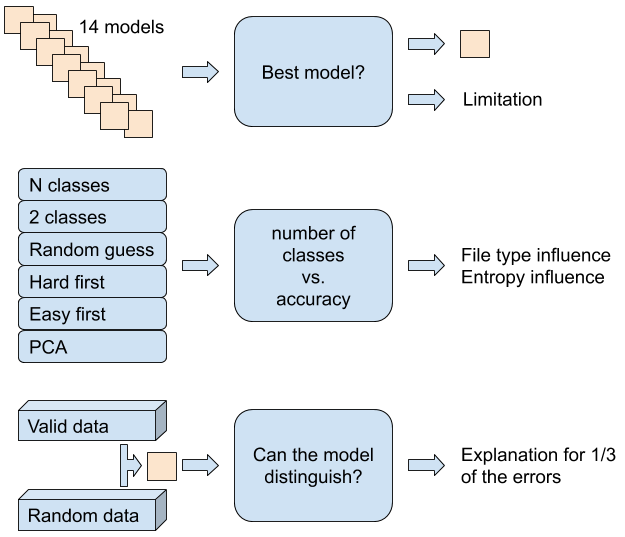
\includegraphics[width=0.8\textwidth]{content/3phases.png}
\caption[Research parts]{\label{fig:steps}Overview of the three parts of the research.}%
\end{figure*}


In this work, only neural networks are taken into account, but other machine learning approaches could also be applied, like Support Vector Machines (SVM) \cite{fitzgerald_using_2012} and k-Nearest Neighbors (kNN) \cite{axelsson_normalised_2010}. This restriction was motivated by the success that neural networks have shown in other fields, like image classification\cite{matan_reading_1992} and speech recognition\cite{graves_speech_2013}.

    %\levelB{Overview}
    % \subChapter{Outline}
% providing an overview of the dissertation or report structure

The remainder of this document is organized as follows.
% \todo{check later}
    Chapter 2 describes some key neural network concepts relevant to this work. 
    Chapter 3 analyses current research on file fragment classification. 
    Chapter 4 address the first research question, comparing the accuracy of fourteen neural network models, mixing convolutional, Long Short-Term Memory (LSTM) and fully-connected layers in the file fragment classification task. The initial goal was to identify the most promising models, but an apparent limit was found on how far these models could be improved.
    Chapter 5 address the second research question, exploring the influence of number of classes on the accuracy of the models, in a attempt to understand the limitations found on the chapter 4. While the number of classes seems to influence the accuracy of the trained model, the choice of which file types are included in the dataset have a bigger impact because file types that contain images or use compression were found to have a expressive negative effect on accuracy.
    Motivated by these results, chapter 6 address the third research question, testing the hypothesis that part of the observed errors are caused by high entropy data misinterpreted as random data. 
    Finally, chapter 7 concludes the research and includes suggestions for future work.


    In the first, the accuracy of some types of neural networks is compared, classifying file fragments taken from the Govdocs1 dataset\cite{garfinkel_bringing_2009}, using their file extensions as class labels.
    Then, the influence of the number of classes on the accuracy of the resulting models is explored. Finally, an experiment is devised to measure, for a given neural network architecture, the number of fragments that have recognizable structures for each file type.


%2
\levelA{\label{chap:background}Background}
This chapter describes some key concepts of neural networks and data carving. Section \ref{sec:feedforward} describes the Multilayer Perceptron, a simple neural network that shows the core main concepts and techniques used in other more complex neural networks. Section \ref{sec:conv} describes the Convolutional Neural Network, a type of neural network actively used in image classification. Section \ref{sec:lstm} describes the Long Short-Term Memory, a neural network that can label sequences of inputs. Section \ref{sec:datacarving} describes how some authors classify existing data carving techniques.

    \levelB{\label{sec:feedforward}Multilayer Perceptron}
    Multilayer Perceptron (MLP) \cite{rosenblatt_perceptron:_1958} is a feedforward artificial neural network with at least three layers, in which all layers are fully-connected, meaning that all nodes of a layer are connected to all nodes of the next. The term feedforward implies that the connections between the nodes of the considered network do not form cycles, thus the layers are processed sequentially in order, without feedback loops.

One of the applications of these networks is classification, where given enough labeled input samples they can be trained to classify the inputs in a closed group of categories, often refered as ``classes''.

The output of each layer is the result of a matrix multiplication of the input and a set of weights plus a bias vector, also subject to an optional activation function, as shown in Equation \ref{eq:mpl}, where $y$ is the output vector of the layer, $x$ is the input vector, $W$ is the set of weights matrix, $b$ is the bias vector, and $a$ is the activation function.

\begin{align}
\label{eq:mpl}     
y &= a.(x.W + b)
\end{align}

The training consists of a search for the weights that would minimize the error between the predicted output and the correct label of the instance. This error function is also known as loss function or cost function. Some authors prefer to distinguish between the two using the term ``loss'' to refer to a single training example and ``cost'' to refer to the average of losses in the training set.

% It is important to notice that the framework used to execute the experiments of this work, Keras, does not apply this distinction and uses the term ``loss'' even when the results refer to an entire set of instances.
% \todo[inline]{implementation detail, move or remove}

An essential characteristic of this cost minimization procedure is that it is not random. Given the high number of parameters that can be adjusted, a random search for the lowest cost would be prohibitively expensive.
% \todo{why? because the number of parameter is really high}
The success of neural networks in several fields and applications would not be possible without the backpropagation algorithm \cite{rumelhart_general_1986}. 
% \todo[inline]{define: backpropagation}
This algorithm uses the gradient of the network formulas to propagate the error in the network's output back to each node, assessing how much each weight contributes to this error, and adjusting its value to minimize the error.

When the neural network output results for multiple classes, it is usual to use one-hot encoding in the input and to apply the softmax function in the last layer of the neural network. Softmax applies the exponential function on the vector and then normalizes it. In one-hot encoding, a value is converted into a vector where the number of elements equals the number of desired classes. Only one of the elements is set to one, corresponding to the class of the instance, while the others are set to zero.

Some relevant loss functions for multi-class neural networks are categorical cross-entropy, binary cross-entropy, and mean squared error. 
Assuming the input of the neural network uses one-hot encoding, categorical cross entropy is $-log(\hat{y}_i)$, where $\hat{y}_i$ is the neural network output for the correct class $i$. Binary cross entropy is similar, but penalizes errors in all classes instead of only the correct one. Mean squared error, like binary cross-entropy, also consider all classes simultaneously, but with a different formula. It is the mean of the results of $(\hat{y}_i - y_i)^2$, where $y$ is the correct vector, $\hat{y}$ is the predicted vector, and $i$ is a vector component, corresponding to a class.

To train the neural network, the dataset may be processed multiple times. Each of those cycles is usually called an epoch. Epochs can be further divided into batches, where the adjustments derived from the backpropagation are applied more frequently.

The training stopping condition is arbitrary. Some choices are to use a fixed number of epochs, to train for a fixed period of time, or to stop after a fixed number of epochs without improvement above certain threshold.

    
    \levelB{\label{sec:conv}Convolutional Neural Network}
    Convolutional networks \cite{lecun_backpropagation_1989} \cite{lecun_convolutional_1995} use a sliding window over the input. The convolutional kernel is a matrix with the size of that window. It process the input matrix dividing it in small parts, processing each part using the same procedure described in the multilayer perceptron section, and concatenating the results of each part. The size of the step used to move the window while processing parts of the input matrix is the stride. If it is equal to the kernel size, the input matrix is divided and processed without overlap. To enforce that the final output has the same size of the input, padding may be used, which is a technique that increases the input matrix size, adding elements to its borders.

One of the advantages of convolutional layers is that the number of trainable parameters is reduced in comparison with a fully connected layer. And the linear transformation that the kernel does is uniformly applied across the entire input.

When used to process images, the input of the convolution is a matrix with two dimensions. But, in other applications, as file fragment classification, it is possible to use a one dimension convolution, since the core concept of the convolutional processing can be understood as a simple division of the input in parts, that are then processed separately, concatenating results at the end, a concept that can be applied on any number of dimensions.
% \todo{why? why not?!?}

After the convolutional layer, sometimes a pooling layer is added. It is a special type of convolution that applies a predetermined operation instead of a matrix multiplication with trainable weights. The two most common operations used in pooling layers are max and average. Max pooling returns the highest number of the values being processed, while average pooling uses the average of these values. Pooling layers offer a fast way to achieve translation invariance \cite{hinton_learning_1987}, which means that the detection of patterns is not affected by where in the input they occur. The drawback is that it introduces information loss, since the output is smaller than the input.
    
    % \levelB{\label{sec:rnn}Recurrent Neural Network}
    % \input{content/3.4-rnn.tex}
    
    \levelB{\label{sec:lstm}Long Short-Term Memory}
    Recurrent Neural Network (RNN) are neural networks where part of the input of a layer uses its previous output.
Long Short-Term Memory \cite{hochreiter_long_1997} (LSTM) is a type of Recurrent Neural Network architecture that addresses the problem of vanishing or exploding gradients through time. This problem occurs in regular RNNs because the signal transmitted from one time-step to another is influenced at each interaction, both on forward and backward propagation phases, limiting the potential interaction between distant time-steps. The solution offered by LSTM introduces the concept of a memory cell, adding gates units to each node. The initial proposal included only input and output gates \cite{hochreiter_long_1997}.
The input gate is responsible for regulating if the cell internal state will be affected by the layer input. Similarly, the output gate regulates if the internal state will influence the output of the layer. The concept of a forget gate was introduced later \cite{gers_learning_1999}, to control whether the internal state of the cell should be reset.

Equations \ref{eq:lstmequationsstart} to \ref{eq:lstmequationsend} describe a typical LSTM network. At each time step $t$, $x_t$ is the input vector, $c_t$ is the cell's internal state and $h_t$ is the output state. Both $c_t$ and $h_t$ influence the next time step as variables $c_{t-1}$ and $h_{t-1}$. The symbol $\circ$ denotes an element wise multiplication.

The result of the forget, input, and output gates is represented by $f_t$, $i_t$, and $o_t$.
In each of the three gates, $W$ is the set of weights to be applied to the input $x$, while $U$ is the set of weights to be applied on the previous time step output, $h_{t-1}$. 
The dimensions of $x$ and $h_{t-1}$ are respectively the chosen dimensions for input and output, while the dimension for $W$ and $U$ are such that the output has the same dimensions of $h_{t-1}$.  Symbol $b$ denotes the bias vector, having the same dimensions of both $h$ and $h_{t-1}$. Symbol $\sigma_g$ denotes the activation function of the gate. Each gate is mathematically equivalent to a fully connected layer where the inputs are the concatenation of the $x$ and $h_{t-1}$ vectors and the output has the same dimensions of $h$.

The activation function usually chosen for the gates is the sigmoid, which gives values in the $[0,1]$ range. If the forget gate $f_t$ results zero for a given component, the corresponding component in the $c_{t-1}$ vector will have no influence on $c_t$ or $h_t$. If all the resulting components of the forget gate are zero, which corresponds to the zero vector, then the previous cell's state $c_{t-1}$ is completely ignored.
Similarly, if the input gate $i_t$ results in a zero component, the corresponding component in the $c_t$ vector will not be influenced by $x$ and $h_{t-1}$.

If all components of $f_t$ and $i_t$ are equal to $1$, then $c_t = c_{t-1} + \sigma_c(x_t W_{c} + h_{t-1} U_{c} + b_c)$, which is the case where $c_t$ is fully influenced by $c_{t-1}$, $x$ and $h_{t-1}$.

The output gate $o_t$ follows a similar pattern, but it regulates how $h_t$ will be influenced by $c_t$.

\begin{align}
\label{eq:lstmequationsstart}     
f_t &= \sigma_g(x_t W_{f} + h_{t-1} U_{f} + b_f) \\
i_t &= \sigma_g(x_t W_{i} + h_{t-1} U_{i} + b_i) \\
o_t &= \sigma_g(x_t W_{o} + h_{t-1} U_{o} + b_o) \\
c_t &= f_t \circ c_{t-1} + i_t \circ \sigma_c(x_t W_{c} + h_{t-1} U_{c} + b_c) \\
\label{eq:lstmequationsend}
h_t &= o_t \circ \sigma_h(c_t)
    \end{align}

% \todo[inline]{conclusion of nn section, conclusion of data carving section, and conclusion of chapter. What could possibly be concluded?!?! In this chapter we will describe y. Y=x. In this chapter we described y.}

    \levelB{\label{sec:datacarving}Data carving}
    Ali \textit{et al.} \cite{ali_review_2018} divide the data carving process into three steps:
    identification, which classifies the file type of individual chunks of data; 
    validation, which includes a list of requirements of a file that are needed for its recovery to be considered successful; and
    reassembling, which attempts to reconstruct the original file.
    
%from pep 2.2, paragrafo 3
Nadeem \cite{nadeem_ashraf_forensic_2013} groups the carving techniques into three generations, each extending the previous one.
%from pep 2.2, paragrafo 4
The first generation is header-footer based carving. It uses file signatures like magic-bytes, headers, and footers to identify the beginning and end of a file.
%from pep 2.2, paragrafo 5
The second generation is structure-based carving, also called ``semantic carving'' or ``deep carving''. It reduces the number of false positives by using file structure knowledge to perform validation.
%from pep 2.2, paragrafo 6
The third generation advances reassembling with methods to deal with fragmentation. It tries to infer relationships and the order between chunks of data based on content and statistical analysis to reassemble the original file.

%from pep 2.2, paragrafo 7
For file type detection, which could be mapped to the identification step in the  process steps of Ali \textit{et al.} \cite{ali_review_2018}, Amirami \textit{et al.} \cite{amirani_new_2008} cite three categories: extension-based identification, magic bytes-based identification, and content-based identification.
In extension-based identification, the content of the file is ignored and only its filename extension is used. Magic bytes-based identification uses signatures, generally a fixed string, usually at the beginning of a file. It is a common strategy that uses header/footer, but not all files adopt it. Content-based identification identifies the file using some statistical modeling of its content.

%from pep 2.2, paragrafo 8
Beebe \textit{et al.} \cite{beebe_sceadan:_2013} identify three content-based approaches to classify file and data types, also referring only to the identification step of the Ali \textit{et al.} \cite{ali_review_2018} data carving process division: semantic parsing, nonsemantic parsing, and machine learning. Semantic parsing relies on the file structure to identify its type. Nonsemantic parsing searches for strings that are commonly found in specific files. Machine learning uses supervised and unsupervised algorithms, like Support Vector Machine (SVM), k-Nearest Neighbors (kNN), and neural networks.

%from pep 2.2, paragrafo 9
A summary of the categorization schemes is depicted in Table \ref{tab:categories}. As Nadeem \cite{nadeem_ashraf_forensic_2013} does not specifically mention machine learning, it is left out of generation classification.

\begin{table*}[!ht]
    \centering
    \caption[Summary of data carving categorization schemes]{Summary of data carving categorization schemes according to other authors}
    \label{tab:categories}
    \begin{tabular}{ l | l | l | c }
      Steps & \multicolumn{2}{|c|}{Techniques}                  & Generation\\
      \hline\hline
      Identification    & extension-based   &                   &   \\
                        \cline{2-3}
                        & magic bytes-based &                   & \multirow{-2}{*}{1\textsuperscript{st}}\\
                        \cline{2-4}
                        & content-based     & semantic          &   \\
                                            \cline{3-3}
                        &                   & non-semantic      & \multirow{-2}{*}{2\textsuperscript{nd}}\\
                                            \cline{3-4}
                        &                   & machine learning  &  --- \\
      \hline
      Validation        &                   &                   & 2\textsuperscript{nd} \\
      \hline
      Reassembling      &                   &                   & 3\textsuperscript{rd}\\
      \hline
    \end{tabular}
\end{table*}



\todo[inline]{incluir seção de conclusão dizendo as estratégias de data carving que serão usadas e os tópicos do background que serão usados}

%3
\levelA{Related work}
\chapter{Related work}
%from pep 2.2, paragrafo 1
Ali et al. \cite{ali_review_2018} divide the data carving process in three steps:
    identification, which classifies the file type of individual chunks of data; 
    validation, which includes a list of requirements of a file that are needed for its recovery to be considered successful; and
    reassembling, which attempts to reconstruct the original file.

%from pep 2.2, paragrafo 3
Nadeem \cite{nadeem_ashraf_forensic_2013} groups the carving techniques in three generations, each extending the previous one.
%from pep 2.2, paragrafo 4
The first generation is a header-footer based carving. It uses file signatures like magic-bytes, headers, and footers to identify the beginning and end of a file.
%from pep 2.2, paragrafo 5
The second generation is structure based carving, also called ``semantic carving'' or ``deep carving''. It reduces the number of false positives by using file structure knowledge to perform validation.
%from pep 2.2, paragrafo 6
The third generation advances reassembling with methods to deal with fragmentation. It tries to infer relationships and order between chunks of data based on content and statistical analysis to reassemble the original file.

%from pep 2.2, paragrafo 7
For file type detection, which could be mapped to the identification step in the  process steps of Ali et al. \cite{ali_review_2018}, Amirami et al. \cite{amirani_new_2008} cite three categories: extension-based identification, magic bytes-based identification, and content-based identification.
In extension-based identification, the content of the file is ignored and only its filename extension is used. Magic bytes-based identification uses signatures, generally a fixed string, usually at the beginning of a file. It is a common strategy that uses header/footer, but not all files adopt it. Content-based identification identifies the file using some statistical modeling of its content.

%from pep 2.2, paragrafo 8
Beebe et al. \cite{beebe_sceadan:_2013} identify three content-based approaches to classify file and data types, also referring only to the identification step of the Ali et al. \cite{ali_review_2018} data carving process division: semantic parsing, nonsemantic parsing, and machine learning. Semantic parsing relies on the file structure to identify its type. Nonsemantic parsing searches for strings that are commonly found in specific files. Machine learning uses supervised and unsupervised algorithms, like Support Vector Machine (SVM), k-Nearest Neighbors (kNN), and Neural Networks (NN).

\todo[inline]{qual a relação de ML com a evolucao de data carving?}

\sigla{NN}{Neural Networks}
\sigla{kNN}{k-Nearest Neighbors}
\sigla{SVM}{Support Vector Machine}

%from pep 2.2, paragrafo 9
A summary of the categorization schemes is depicted on Table \ref{tab:categories}. As Nadeem \cite{nadeem_ashraf_forensic_2013} does not specifically mention machine learning, it is left out of generation classification.

\begin{table*}[!ht]
    \centering
    \caption{Data carving categories}
    \label{tab:categories}
    \begin{tabular}{ l | l | l | c }
      \multicolumn{3}{l|}{Steps}                                 & Generation\\
      \hline\hline
      Identification    & extension-based   &                   &   \\
                        \cline{2-3}
                        & magic bytes-based &                   & \multirow{-2}{*}{1\textsuperscript{st}}\\
                        \cline{2-4}
                        & content-based     & semantic          &   \\
                                            \cline{3-3}
                        &                   & non-semantic      & \multirow{-2}{*}{2\textsuperscript{nd}}\\
                                            \cline{3-4}
                        &                   & machine learning  &  --- \\
      \hline
      Validation        &                   &                   & 2\textsuperscript{nd} \\
      \hline
      Reassembling      &                   &                   & 3\textsuperscript{rd}\\
      \hline
    \end{tabular}
\end{table*}



\todo[inline]{diferenças entre este trabalho e outros: dados, metodologia e resultados}

\todo[inline]{qual a acurácia das ferramentas tradicionais? e das técnicas apresentadas em papers?}
%from pep 4, paragrafo 2
Several authors reviewed  available data carving tools
\cite{ali_review_2018}
\cite{qiu_new_2014}
\cite{nadeem_ashraf_forensic_2013}
\cite{roux_reconstructing_2008}, 
but the tool listing from Ali \textit{et al.} \cite{ali_review_2018} was found to be the most comprehensive one. Among the listed tools, only Foremost \cite{kendall_foremost_2019}, Scalpel \cite{richard_iii_scalpel:_2005}, and PhotoRec \cite{grenier_photorec_2019} support a wide range of file formats. For example, Photorec supports more than 300 file types.

%from pep 4, paragrafo 1
The available data carving tools generally do not take advantage of the latest techniques that research on the field offers, often still relying on header/footer identification and providing limited reassembling capabilities.
%from pep 2, paragrafo 11
According to Ali \textit{et al.} \cite{ali_review_2018}, artificial intelligence techniques are found to be not fully utilized in this field.

Comparing the accuracy between research papers and available software is difficult because, as they rely on header and footer identification, their performance would be more properly compared to whole file classification instead of file fragment classification, the latter being a harder problem.

%%%%%%%%%%%%%%%%%%%%%%%%%%%%%%%%%%%%%%%%%%%%%%%%
% indicating a problem, controversy or a knowledge gap in the field of study

% identification
% validation
% fragmentation
%from pep 4, paragrafo 5
Each of the steps cited by Ali et al. \cite{ali_review_2018} for the data carving process deals with a main challenge. The identification step is responsible for classifying the file type. The quantity and diversity of file types, together with the accuracy and precision of the results, are the main challenges in identification. The second step, validation, also deals with classification, but it is a complementary step to the previous one to reduce false positives, often using a different technique. For that reason, validation challenges are similar to the identification ones. The last step, reassembling, has fragmentation as its main challenge.

% - more file types
% - reassembling
% - new carvers easier
%from pep 4, paragrafo 4
The work of Hiester \cite{hiester_file_2018} has shown that LSTM neural networks have good potential in the data carving field. But, as happens with studies applying LSTM models to speech recognition, where many researchers have contributed with different models, adjustments, modifications, and innovations, also in the field of data carving field it is important to further advance the research. Important aspects that require attention include support for a wider range of file types, handle fragmentation through reassembling, and make the task of supporting the carving of a new file type easier.

% datasets and file structures

% challenge: reveal structures in the file
% from pep 4, paragrafo 6
% In the current proposal, a new type of challenge is introduced. Instead of using previous knowledge of the file structure to improve carving results, \textbf{would be possible to do the inverse and use insights from the carving process to reveal structures in the file?}

% challenge: reveal structures in the file
%from pep 4, paragrafo 7
% For example, suppose a file has a fixed size field, a 32 bit unsigned integer representing a datetime value. 
% For that type of field, the insight may come in the form of an expected range. Still using the datetime example, a possible outcome would be the observation that a certain kind of file always presents that field value inside some range, that coincides with a range often observed in datetime fields. That does not prove the unknown field to be a datetime but suggests that direction.

% challenge: reveal structures in the file
%from pep 4, paragrafo 8
% Few structures are so simple as a group of fixed sized fields. It is very common, for example, to use a field to specify the length of the next field. Another type of complexity increase occurs when the value of a field establishes which specification should be used in the remaining of the file, changing which fields should be expected next.

% challenge: reveal structures in the file
% %from pep 4, paragrafo 9
% The greater the complexity of an unknown file structure is, the more difficult it is to unravel its specification, but also the more useful it is to count with tools that automatize that task. Otherwise, the only option is to manually write the specification or the parser, possibly relying on reverse engineering techniques.

% challenge: reveal structures in the file
%from pep 4, paragrafo 10
% The direct utility of the discovery of file type structures is the extraction of values from its fields. This information has value for itself, but could also be used to improve validation and even reassembling.

% challenge: datasets
%from pep 4, paragrafo 11
% Another concern that can be explored and is pertinent to possibly all of the previous studies combining neural networks and data carving is that their datasets and results may not reflect the same situations that would be faced on a real forensic scenario, where the distribution of file types may be different and the occurrence of unknown and untreated formats may be frequent. Therefore, more realistic datasets are important to improve research validation. 
%%%%%%%%%%%%%%%%%%%%%%%%%%%%%%%%%%%%%%%%%%%%%%%%



%from pep 2.1, paragrafos 12, 13
Amirami et al.  \cite{amirani_new_2008} appear to be the first 
to provide a viable alternative to classical data carving tools using a neural network approach. Two previous works were found using neural networks with data carving related goals, by Dunhan et al. \cite{dunham_classifying_2005} and Harris \cite{harris_using_2007}, but the first worked with encrypted files only and the second did not achieve good results.

%from pep 2.1, paragrafos 14
Amirami et al.  \cite{amirani_new_2008} used Principal Component Analysis (PCA) as input for a 5 layer feed-forward auto-associative unsupervised neural network to do feature extraction and a 3 layer Multi Layer Perceptron (MLP) to perform classification. They used a similar approach in 2013 \cite{amirani_feature-based_2013}.
\sigla{PCA}{Principal Component Analysis}
\sigla{MLP}{Multi Layer Perceptron}

%from pep 2.1, paragrafos 16,17,18
Other works were found applying neural networks to perform data carving, also using some form of dimensionality reduction as PCA. Ahmed et al. \cite{ahmed_content-based_2010}\cite{ahmed_fast_2011} used byte frequency, 
Penrose et al. \cite{penrose_approaches_2013} used compression rate,
and Maslim et al. \cite{maslim_distributed_2014} used PCA, as did Amirami et al.  \cite{amirani_new_2008}.

%from pep 2.1, paragrafos 15
Xu and Dong \cite{xu_reassembling_2009} used a neural network as a cluster reassembling technique for JPEG image fragments.

%from pep 2.1, paragrafos 19
Hiester \cite{hiester_file_2018} apparently was the first to not resort to dimensionality reduction and also the first to utilize a LSTM network to perform file fragment classification. He compared results using three types of neural networks: feedforward, convolutional, and long short-term memory. The goal was to classify the data type of individual sectors (512 bytes), considering four file types: CSV, XML, JPG and GIF.

% Table \ref{tab:datacarvingstudies} summarizes the  machine learning techniques used in each data carving study.
% \begin{table}[!ht]
\caption{Data carving studies using machine learning}
\label{tab:datacarvingstudies}
\begin{tabular}{l|c|c|c|c}

                                & \multicolumn{4}{c}{Technique} \\ \hline
Study                                     & SVM    & kNN    & NN   & ELM   \\ \hline
\hline
Dunham et al. \cite{dunham_classifying_2005}       &        &        & x    &       \\ \hline
Harris \cite{harris_using_2007}             &        &        & x    &       \\ \hline
Amirani et al. \cite{amirani_new_2008}              &        &        & x    &       \\ \hline
Xu and Dong \cite{xu_reassembling_2009}          &        &        & x    &       \\ \hline
Ahmed et al. \cite{ahmed_content-based_2010}      &        &        & x    &       \\ \hline
Axelsson \cite{axelsson_normalised_2010}      &        & x      &      &       \\ \hline
Conti et al. \cite{conti_automated_2010}          &        & x      &      &       \\ \hline
Ahmed et al. \cite{ahmed_fast_2011}               & x      & x      & x    &       \\ \hline
Gopal et al. \cite{gopal_statistical_2011}        & x      & x      &      &       \\ \hline
Luigi and Stefano \cite{luigi_file_2011}               & x      &        &      &       \\ \hline
Sportiello and Zanero \cite{sportiello_file_2011}          & x      &        &      &       \\ \hline
Fitzgerald et al. \cite{fitzgerald_using_2012}         & x      &        &      &       \\ \hline
Sportiello and Zanero \cite{sportiello_context-based_2012} & x      &        &      &       \\ \hline
Amirani et al. \cite{amirani_feature-based_2013}    & x      &        & x    &       \\ \hline
Beebe et al. \cite{beebe_sceadan:_2013}           & x      &        &      &       \\ \hline
Penrose et al. \cite{penrose_approaches_2013}       &        &        & x    &       \\ \hline
Qiu et al. \cite{qiu_new_2014}                  & x      &        &      &       \\ \hline
Maslim et al. \cite{maslim_distributed_2014}       &        &        & x    &       \\ \hline
Zhang et al. \cite{zhang_svm_2016}                & x      &        &      & x      \\ \hline
Ali et al. \cite{ali_classification_2018}       &        &        &      & x     \\ \hline
Hiester \cite{hiester_file_2018}             &        &        & x    &       \\ %\hline
\end{tabular}
\end{table}


    \label{sec:relatedwork}
    % \levelB{From PEP}
    The early studies on data carving used private datasets

\cite{karresand_file_2006} \cite{veenman_statistical_2007} \cite{erbacher_identification_2007} \cite{moody_sadi-statistical_2008} \cite{calhoun_predicting_2008} \cite{li_novel_2010} \cite{conti_automated_2010} \cite{kattan_gp-fileprints:_2010},
making it difficult to compare the results of different studies. In 2009, Garfinkel \textit{et al.} \cite{garfinkel_bringing_2009} published the Govdocs1 dataset with 1 million files (a small amount of those files was removed later, for legal reasons). While some of the later works on the field still use private datasets, the Govdocs1 dataset has become the most used choice in studies related to data carving. Therefore, this related work summary focuses on studies on file fragment classification that used the Govdocs1 dataset.

Depending on the objective, the focus of each study may either be whole file classification or file fragment classification. The whole file classification is generally an easier task because most file types, even those with high entropy and low compression rates, have well-structured headers, with easily recognizable patterns.

Most of the early work in this field used some form of dimensionality reduction in the input data before performing classification, as byte frequency distribution 
\cite{karresand_oscarfile_2006} \cite{harris_using_2007} \cite{amirani_new_2008} \cite{ahmed_content-based_2010} \cite{ahmed_fast_2010} \cite{sportiello_context-based_2012} \cite{amirani_feature-based_2013} \cite{qiu_new_2014} \cite{maslim_distributed_2014} \cite{ali_classification_2018}, compression rate \cite{axelsson_normalised_2010} \cite{penrose_approaches_2013}, and various statistical techniques \cite{veenman_statistical_2007} \cite{erbacher_identification_2007} \cite{moody_sadi-statistical_2008} \cite{calhoun_predicting_2008} \cite{li_novel_2010} \cite{kattan_gp-fileprints:_2010} \cite{gopal_statistical_2011}. The usage of raw bytes as input is recently becoming more popular \cite{hiester_file_2018} \cite{chen_file_2018} \cite{wang_sparse_2018} \cite{wang_file_2018} \cite{vulinovic_neural_2019},
especially in studies applying machine learning techniques, which seems to be a rising trend in the last ten years.

Each of the following studies chose a subset of file types from the Govdocs1 dataset, splitting this subset further into training and validation parts. The training dataset was used to train the machine learning solution to classify file fragments, while the validation dataset was used to verify how accurately the model could predict the type of the file from which the fragment was extracted from.

% \todo[inline]{figure explaining the splitting and usage of govdocs1}

Axelsson \cite{axelsson_normalised_2010} used the normalized compression distance as an input feature to a kNN algorithm, picking pairs of 512-byte fragments, compressing them with the bzip2 algorithm and comparing the length of the results.
He got an average accuracy of around 34\% using 28 file types.

Fitzgerald \textit{et al.} \cite{fitzgerald_using_2012}  used an SVM classifier with various statistical measures as input features, including unigram and bigram histogram counts, Shannon entropy, and compression length.
Omitting the first and the last fragments of each file, they got an average accuracy of 49.1\% using 24 file types.

Beebe \textit{et al.} \cite{beebe_sceadan:_2013}
compared various measures of complexity and byte frequency distributions of 512-byte fragments as input features to an SVM algorithm. They used 8 data types, txt, base64, base85, urlencoded, fat fs data, ntfs fs data, ext fs data, aes256, and
30 file types
from the Govdocs1 dataset and some other sources (19 are at least partially from the Govdocs1 dataset). They got an average accuracy of 73.4\% combining unigram and bigrams as input features.

Chen \textit{et al.} \cite{chen_file_2018}
used a Convolutional Neural Network (CNN) with five convolutional layers and 3 fully connected layers to classify fragments of 4096 bytes, converting each fragment into a 64x64 grayscale picture.
They got an average accuracy of 70.9\% using 16 file types.

Hiester \cite{hiester_file_2018} apparently was the first to use an LSTM network to perform file fragment classification. He compared the results of three types of neural networks: feedforward, convolutional, and LSTM. He used four file types from the Govdocs1 dataset.
Each bit of a 512-byte fragment was translated into two features, resulting in 8192 features per block (512*8*2). The first and last sectors of each file in the training set were discarded. In the experiments, the datasets were limited to one gigabyte to fit in memory. He got an average accuracy of 98\% using an LSTM network, 73\% using CNN, and 76\% using MLP.

Wang \textit{et al.} \cite{wang_sparse_2018} 
used sparse dictionaries for n-grams to extract features of 512-byte fragments, using this as input to an SVM classifier.
They got an average accuracy of 61.3\% using 18 file types.

Wang \textit{et al.} \cite{wang_file_2018}  
compared CNN, SVM, kNN, and XGboost, with fragments of different sizes, converting each byte to a 256-length vector (one-hot encoding). The CNN combined three parallel convolutional layers of widths 4, 8 and 16.
They used 20 file types from the Govdocs1 dataset.
Using CNN, they got an average accuracy of around 68\% with 512-byte fragments, and around 78\% with 4096-byte fragments.

Vulinović \textit{et al.} \cite{vulinovic_neural_2019}
compared a CNN with MLP, using 512 raw bytes as the CNN input, and byte histograms as input to the MLP.
Using 18 file types, they got a macro average F1-score of 61\% using CNN and 81\% using MLP.

Table \ref{tab:datacarvingstudies} summarizes 
the results of file fragment classification studies using Govdocs1 dataset and Table \ref{tab:studiesfiletypes}
lists the file types used in each study.

\begin{table*}[!ht]
\caption{\label{tab:datacarvingstudies}File fragment classification studies using the Govdocs1 dataset}
\resizebox{\linewidth}{!}{%
\begin{tabular}{|l|l|l|l|l|l|l|l|l|l|l|}
\hline
Study                                          & SVM & kNN & NN   & Dataset       & Raw   & Fragment & Number   & Accuracy   & F1-score  \\
                                               &     &     &      &               & bytes & size     & of types &            &           \\ \hline
Axelsson \cite{axelsson_normalised_2010}       &     & x   &      & Govdocs1      & No    & 512      & 28       & 34\%       &           \\ \hline
Fitzgerald et al. \cite{fitzgerald_using_2012} & x   &     &      & Govdocs1      & No    & 512      & 24       & 49\%       & 48\%      \\ \hline
Beebe et al. \cite{beebe_sceadan:_2013}        & x   &     &      & Govdocs1 +    & No    & 512      & 38       & 73\%       &           \\
                                               &     &     &      & other sources &       &          &          &            &           \\ \hline
Hiester \cite{hiester_file_2018}               &     &     & MLP  & Govdocs1      & Yes   & 512      & 4        & 77\%       &           \\
                                               &     &     & CNN  &               &       &          &          & 73\%       &           \\
                                               &     &     & LSTM &               &       &          &          & 98\%       &           \\ \hline
Chen \cite{chen_file_2018}                     &     &     & CNN  & Govdocs1      & Yes   & 4096     & 16       & 71\%       &           \\ \hline
Wang \cite{wang_sparse_2018}                   & x   &     &      & Govdocs1      & Yes   & 512      & 18       & 61\%       & 61\%      \\ \hline
Wang \cite{wang_file_2018}                     &     &     & CNN  & Govdocs1      & Yes   & 512      & 20       & 68\%       &           \\
                                               &     &     &      &               &       & 4096     &          & 78\%       &           \\ \hline
Vulinovic \cite{vulinovic_neural_2019}         &     &     & MLP  & Govdocs1      & Yes   & 512      & 18       &            & 81\%      \\
                                               &     &     & CNN  &               &       &          &          &            & 61\%      \\ \hline
\end{tabular}}
\end{table*}


\begin{table}[!ht]
    \centering
    \caption{The Govdocs1 dataset and file types used in each study}
    \label{tab:studiesfiletypes}
\footnotesize
\begin{tabular}{|l|l|l|l|l|l|l|l|l|l|l|l|}
\hline
Extension & Number of files & Number of blocks
                                            & \rotatebox{90}{this study}
                                                & \rotatebox{90}{Axelsson \cite{axelsson_normalised_2010}}
                                                    & \rotatebox{90}{Fitzgerald et al. \cite{fitzgerald_using_2012}}
                                                        & \rotatebox{90}{Beebe et al. \cite{beebe_sceadan:_2013}}
                                                            & \rotatebox{90}{Hiester \cite{hiester_file_2018}}
                                                                & \rotatebox{90}{Chen \cite{chen_file_2018}}
                                                                    & \rotatebox{90}{Wang \cite{wang_sparse_2018}}
                                                                        & \rotatebox{90}{Wang \cite{wang_file_2018}}
                                                                            & \rotatebox{90}{Vulinovic \cite{vulinovic_neural_2019}}
                                                   \\ \hline
                                                      \hline
pdf       & 231232          & 268071071     & x & x & x & x &   & x & x & x & x   \\ \hline
html      & 214568          & 25710908      & x & x & x & x &   & x & x & x & x   \\ \hline
jpg       & 109233          & 73242253      & x & x & x & x & x & x & x & x & x   \\ \hline
txt       & 78286           & 99435540      & x &   & x & x &   &   & x & x & x   \\ \hline
doc       & 76616           & 60654930      & x & x & x & x &   & x & x & x & x   \\ \hline
xls       & 62635           & 58718224      & x & x & x & x &   & x & x & x & x   \\ \hline
ppt       & 49702           & 251210471     & x & x & x & x &   & x & x & x & x   \\ \hline
gif       & 36302           & 5962516       & x & x & x & x & x & x & x & x & x   \\ \hline
xml       & 33458           & 16954875      & x & x & x & x & x & x & x & x & x   \\ \hline
ps        & 22015           & 56547464      & x & x & x & x &   &   & x & x & x   \\ \hline
csv       & 18360           & 6843009       & x & x & x & x & x & x & x & x & x   \\ \hline
gz        & 13725           & 17748905      & x & x & x & x &   & x & x & x & x   \\ \hline
log       & 9976            & 8467819       & x &   &   & x &   & x &   & x &     \\ \hline
eps       & 5191            & 5756138       & x & x &   &   &   &   &   &   &     \\ \hline
unk       & 5186            & 2983922       &   &   &   &   &   &   &   & x &     \\ \hline
png       & 4125            & 2207489       & x & x & x & x &   & x & x & x & x   \\ \hline
swf       & 3476            & 3798321       & x & x & x &   &   &   & x & x & x   \\ \hline
dbase3    & 2601            & 38972         & x &   &   &   &   &   &   & x &     \\ \hline
pps       & 1619            & 7432480       & x & x & x &   &   &   &   &   &     \\ \hline
rtf       & 1125            & 958239        & x &   & x &   &   & x & x & x & x   \\ \hline
kml       & 993             & 309422        & x &   &   &   &   &   &   &   &     \\ \hline
kmz       & 943             & 549462        & x &   &   &   &   &   &   &   &     \\ \hline
text      & 839             & 1527118       &   & x &   &   &   & x &   &   &     \\ \hline
hlp       & 659             & 8692          & x &   &   &   &   &   &   &   &     \\ \hline
f         & 602             & 94543         & x &   &   &   &   &   &   & x &     \\ \hline
sql       & 462             & 244634        & x & x & x &   &   &   &   &   &     \\ \hline
wp        & 364             & 87643         & x &   &   &   &   &   &   &   &     \\ \hline
dwf       & 299             & 85500         & x &   &   &   &   &   &   &   &     \\ \hline
java      & 292             & 14530         & x & x & x & x &   & x &   & x &     \\ \hline
pptx      & 215             & 1151796       & x & x & x & x &   &   & x &   & x   \\ \hline
% fits      & 182             & 678128        &   &   &   &   &   &   &   &   &     \\ \hline
% tmp       & 180             & 28426         &   &   &   &   &   &   &   &   &     \\ \hline
tex       & 163             & 10520         &   &   & x &   &   &   &   &   &     \\ \hline
docx      & 163             & 65969         &   & x & x & x &   & x & x &   & x   \\ \hline
% troff     & 110             & 8020          &   &   &   &   &   &   &   &   &     \\ \hline
bmp       & 72              & 62686         &   & x & x & x &   &   &   &   &     \\ \hline
% sgml      & 62              & 44138         &   &   &   &   &   &   &   &   &     \\ \hline
% gls       & 60              & 517           &   &   &   &   &   &   &   &   &     \\ \hline
pub       & 55              & 1421          &   & x &   &   &   &   &   &   &     \\ \hline
xlsx      & 37              & 12910         &   & x & x & x &   &   & x &   & x   \\ \hline
% fm        & 25              & 6717          &   &   &   &   &   &   &   &   &     \\ \hline
zip       & 10              & 31525         &   & x & x &   &   &   &   &   &     \\ \hline
ttf       & 10              & 1540          &   & x &   &   &   &   &   &   &     \\ \hline
xbm       & 8               & 578           &   & x &   &   &   &   &   &   &     \\ \hline
% wk1       & 7               & 6493          &   &   &   &   &   &   &   &   &     \\ \hline
% sys       & 7               & 15            &   &   &   &   &   &   &   &   &     \\ \hline
% ileaf     & 4               & 1656          &   &   &   &   &   &   &   &   &     \\ \hline
% exported  & 3               & 324           &   &   &   &   &   &   &   &   &     \\ \hline
% data      & 3               & 1733          &   &   &   &   &   &   &   &   &     \\ \hline
% odp       & 2               & 2384          &   &   &   &   &   &   &   &   &     \\ \hline
% mac       & 2               & 0             &   &   &   &   &   &   &   &   &     \\ \hline
% lnk       & 2               & 2             &   &   &   &   &   &   &   &   &     \\ \hline
js        & 2               & 36            &   & x &   &   &   &   &   &   &     \\ \hline
% g3        & 2               & 498           &   &   &   &   &   &   &   &   &     \\ \hline
% chp       & 2               & 73            &   &   &   &   &   &   &   &   &     \\ \hline
% 123       & 2               & 434           &   &   &   &   &   &   &   &   &     \\ \hline
% wk3       & 1               & 229           &   &   &   &   &   &   &   &   &     \\ \hline
% vrml      & 1               & 660           &   &   &   &   &   &   &   &   &     \\ \hline
% squeak    & 1               & 25354         &   &   &   &   &   &   &   &   &     \\ \hline
% py        & 1               & 480           &   &   &   &   &   &   &   &   &     \\ \hline
% pst       & 1               & 20            &   &   &   &   &   &   &   &   &     \\ \hline
% icns      & 1               & 0             &   &   &   &   &   &   &   &   &     \\ \hline
% bin       & 1               & 7             &   &   &   &   &   &   &   &   &     \\ \hline
\end{tabular}
\end{table}



In the early stages of the study described in this dissertation, the search for a better classification technique was assumed to be the best approach to improve file fragment classification results. This assumption seems to be also present in the many of the reviewed works, as their approaches suggest. This study found indications that this assumption may be false, and that further improvement may require a review of the labeling system commonly used, that uses the extension of the file as the label for all its fragments.

\todo[inline]{Isto vai ser retomado em algum momento? Nem que seja na conclusão. (Estou lendo e não vi ainda, mas deixei o comentário para você verificar).}
    % \levelB{Current data carving tools}
    %from pep 4, paragrafo 2
Several authors reviewed  available data carving tools
\cite{ali_review_2018}
\cite{qiu_new_2014}
\cite{nadeem_ashraf_forensic_2013}
\cite{roux_reconstructing_2008}, 
but the tool listing from Ali \textit{et al.} \cite{ali_review_2018} was found to be the most comprehensive one. Among the listed tools, only Foremost \cite{kendall_foremost_2019}, Scalpel \cite{richard_iii_scalpel:_2005}, and PhotoRec \cite{grenier_photorec_2019} support a wide range of file formats. For example, Photorec supports more than 300 file types.

%from pep 4, paragrafo 1
The available data carving tools generally do not take advantage of the latest techniques that research on the field offers, often still relying on header/footer identification and providing limited reassembling capabilities.
%from pep 2, paragrafo 11
According to Ali \textit{et al.} \cite{ali_review_2018}, artificial intelligence techniques are found to be not fully utilized in this field.

Comparing the accuracy between research papers and available software is difficult because, as they rely on header and footer identification, their performance would be more properly compared to whole file classification instead of file fragment classification, the latter being a harder problem.

    % \levelB{Data carving challenges}
    % %%%%%%%%%%%%%%%%%%%%%%%%%%%%%%%%%%%%%%%%%%%%%%%%
% indicating a problem, controversy or a knowledge gap in the field of study

% identification
% validation
% fragmentation
%from pep 4, paragrafo 5
Each of the steps cited by Ali et al. \cite{ali_review_2018} for the data carving process deals with a main challenge. The identification step is responsible for classifying the file type. The quantity and diversity of file types, together with the accuracy and precision of the results, are the main challenges in identification. The second step, validation, also deals with classification, but it is a complementary step to the previous one to reduce false positives, often using a different technique. For that reason, validation challenges are similar to the identification ones. The last step, reassembling, has fragmentation as its main challenge.

% - more file types
% - reassembling
% - new carvers easier
%from pep 4, paragrafo 4
The work of Hiester \cite{hiester_file_2018} has shown that LSTM neural networks have good potential in the data carving field. But, as happens with studies applying LSTM models to speech recognition, where many researchers have contributed with different models, adjustments, modifications, and innovations, also in the field of data carving field it is important to further advance the research. Important aspects that require attention include support for a wider range of file types, handle fragmentation through reassembling, and make the task of supporting the carving of a new file type easier.

% datasets and file structures

% challenge: reveal structures in the file
% from pep 4, paragrafo 6
% In the current proposal, a new type of challenge is introduced. Instead of using previous knowledge of the file structure to improve carving results, \textbf{would be possible to do the inverse and use insights from the carving process to reveal structures in the file?}

% challenge: reveal structures in the file
%from pep 4, paragrafo 7
% For example, suppose a file has a fixed size field, a 32 bit unsigned integer representing a datetime value. 
% For that type of field, the insight may come in the form of an expected range. Still using the datetime example, a possible outcome would be the observation that a certain kind of file always presents that field value inside some range, that coincides with a range often observed in datetime fields. That does not prove the unknown field to be a datetime but suggests that direction.

% challenge: reveal structures in the file
%from pep 4, paragrafo 8
% Few structures are so simple as a group of fixed sized fields. It is very common, for example, to use a field to specify the length of the next field. Another type of complexity increase occurs when the value of a field establishes which specification should be used in the remaining of the file, changing which fields should be expected next.

% challenge: reveal structures in the file
% %from pep 4, paragrafo 9
% The greater the complexity of an unknown file structure is, the more difficult it is to unravel its specification, but also the more useful it is to count with tools that automatize that task. Otherwise, the only option is to manually write the specification or the parser, possibly relying on reverse engineering techniques.

% challenge: reveal structures in the file
%from pep 4, paragrafo 10
% The direct utility of the discovery of file type structures is the extraction of values from its fields. This information has value for itself, but could also be used to improve validation and even reassembling.

% challenge: datasets
%from pep 4, paragrafo 11
% Another concern that can be explored and is pertinent to possibly all of the previous studies combining neural networks and data carving is that their datasets and results may not reflect the same situations that would be faced on a real forensic scenario, where the distribution of file types may be different and the occurrence of unknown and untreated formats may be frequent. Therefore, more realistic datasets are important to improve research validation. 
%%%%%%%%%%%%%%%%%%%%%%%%%%%%%%%%%%%%%%%%%%%%%%%%



%4
\levelA{Exploratory research of models based on accuracy}
\label{sec:evalmodels}

    % \levelB{Objective}
In this research, different neural networks are trained and validated at the file fragment identification task. Their accuracy is then compared, to identify which models should be considered or disregarded.


    \levelB{Method}
    % \todo[inline]{include method figure}

%\levelB{Dataset sampling}
This study uses the Govdocs1 dataset \cite{garfinkel_bringing_2009}, which was fully downloaded and then organized by file extension.
This dataset has files with 63 different extensions. The 33 extensions with less than 200 files were discarded, to ensure the training and validation dataset would have at least 100 files of each file type.
The  ``text'' and ``unk'' extensions were discarded because examination showed that files with these extensions use multiple formats and they do not correspond to a single file type.
The remaining 28 extensions are listed in Table \ref{tab:studiesfiletypes}.

To select a sample instance from the Govdocs1 dataset, first, a random file is selected among those available, without replacement. Then, a block from this file is randomly selected. After all files have participated in the process, the process may be repeated as long as necessary. This way, all files are considered and the classes are easily balanced.
This contrasts with the sampling technique applied in other works, where all the sectors are grouped before sampling, which may lead to an imbalance between classes.

%\levelB{Inputs}
The input features of the neural network for each instance are a 512x256 matrix representing only one block of 512 bytes of a random file of the dataset. Each of the 512 bytes is one-hot encoded, meaning that its value is converted into a vector with 256 elements, with only one of them set to 1, corresponding to the value of the byte, while the others are set to zero.

%\levelB{Outputs}
The output of the neural network for a given instance is a vector with a size equal to the number of classes, subject to a softmax function, which applies the exponential function on the vector and then normalizes it. Each value will represent the predicted probability that the instance belongs to a specific class.

%\levelB{Models}
The neural networks under consideration used different combinations of convolutional, max pooling, LSTM, and fully connected layers, applying categorical cross-entropy as the loss function. Binary cross-entropy and mean squared error were considered during initial tests, but categorical cross-entropy gave faster training times.

Fourteen neural network models participated in this evaluation.
Their names indicate the types of layers that compose their architecture, using the letter ``C'' to indicate a convolutional layer, ``D'' to indicate a dense layer, also called fully-connected, ``L'' to indicate an LSTM layer, and ``M'' to indicate a max pooling layer. The convolutional layers do not use padding.
Table \ref{tab:models} lists the parameters of the models, which can be analyzed in more detail in the code repository \footnote{http://github.com/atilaromero/carving-experiments}. One of then, ``D'' is a simple single-layer perceptron. Two of them, ``LD'' and ``LL'', use LSTM layers without convolutional layers, while three of them, ``CD'', ``CM'', and ``CCM'', use convolutional layers without LSTM layers. Eight models, ``CL'', ``CML'', ``CLL'', ``CLD'', ``CCL'', ``CCLL'', ``CMCML'', and ``CMCMLL'', combine convolutional layers and LSTM layers. 

\newcommand{\paint}{\cellcolor{gray!25}}
\begin{table}[!ht]
    \centering
    \footnotesize
    \caption{14 models trained on 30 classes}
    \label{tab:models}
\begin{tabular}{l||l|l|l||l|l|l||l|l||l}
\hline
Model  & \multicolumn{3}{l||}{Convolutional layers} & \multicolumn{3}{l||}{Max pooling} & \multicolumn{2}{l||}{LSTM} & Dense  \\ \hline
       & output       & window       & stride      & pool    & stride    & channel    & output     & return       & output \\ 
       & size         & size         & length      & size    & length    & first      & size       & sequences    & size   \\ \hline
                                                                                                                              \hline
D      & \paint       & \paint       &     \paint  & \paint  &  \paint   & \paint     & \paint     & \paint       & 30     \\ \hline
LD     & \paint       & \paint       &     \paint  & \paint  &  \paint   & \paint     & 32         & no           & 30     \\ \hline
LL     & \paint       & \paint       &     \paint  & \paint  &  \paint   & \paint     & 32         & yes          & \paint \\ 
       & \paint       & \paint       &     \paint  & \paint  &  \paint   & \paint     & 32         & no           & \paint \\ \hline
CD     & 64           & 64           & 8           & \paint  &  \paint   & \paint     & \paint     & \paint       & 30     \\ \hline
CM     & 30           & 32           & 1           & 481     & 1         & no         &  \paint    & \paint       & \paint \\ \hline
CCM    & 30           & 32           & 1           &         &           &            & \paint     & \paint       & \paint \\ 
       & 30           & 2            & 2           & 240     & 1         & no         & \paint     & \paint       & \paint \\ \hline
CL     & 30           & 32           & 32          & \paint  &  \paint   & \paint     & 30         & no           & \paint \\ \hline
CML    & 32           & 32           & 32          & 2       & 2         & yes        & 30         & no           & \paint \\ \hline
CLL    & 32           & 32           & 32          & \paint  &  \paint   & \paint     & 64         & yes          & \paint \\ 
       &              &              &             & \paint  &  \paint   & \paint     & 30         & no           & \paint \\ \hline
CLD    & 256          & 16           & 16          & \paint  &  \paint   & \paint     & 128        & no           & 30     \\ \hline
CCL    & 128          & 8            & 8           & \paint  &  \paint   & \paint     &            &              & \paint \\ 
       & 64           & 8            & 8           & \paint  &  \paint   & \paint     & 30         & no           & \paint \\ \hline
CCLL   & 128          & 8            & 8           & \paint  &  \paint   & \paint     & 64         & yes          & \paint \\ 
       & 64           & 8            & 8           & \paint  &  \paint   & \paint     & 30         & no           & \paint \\ \hline
CMCML  & 128          & 8            & 8           & 2       & 2         & yes        &            &              & \paint \\ 
       & 64           & 8            & 8           & 2       & 2         & yes        & 30         & no           & \paint \\ \hline
CMCMLL & 128          & 8            & 8           & 2       & 2         & yes        & 64         & yes          & \paint \\ 
       & 64           & 8            & 8           & 2       & 2         & yes        & 30         & no           & \paint \\ \hline
\end{tabular}
\end{table}

%optimization
All the training sessions used the Adam \cite{kingma_adam:_2014}
optimization algorithm to guide backpropagation, which was selected because it showed good learning speed in the preliminary tests without requiring fine-tuning of parameters.

% Constraints
The models were trained until no further improvement was observed in the last 10 epochs, using categorical cross-entropy loss.

After the 14 models were compared, one of the models with best accuracy results and faster training time, ``CLD'', was chosen to have its results compared with other works, using a longer training session than those used to assess the 14 models.

Using this extended training parameters, the ``CLD'' model was trained with the 28 file types used in the first stage. Then, a different model was built from scratch using the same file types of each of the most recent works listed in Table \ref{tab:datacarvingstudies}: 
Hiester \cite{hiester_file_2018}, 
Chen \textit{et al.} \cite{chen_file_2018},
Wang \textit{et al.} \cite{wang_sparse_2018},
Wang \textit{et al.} \cite{wang_file_2018},
and
Vulinović \textit{et al.} \cite{vulinovic_neural_2019}.

This comparison has three important restrictions.
Chen used 4096 bytes for the block size, while this work used 512 bytes only.
Vulinović got an F1-score of 81\% for the Multilayer Perceptron (MLP) fed with byte histograms, a better result than the one obtained with a Convolutional Neural Network (CNN) fed with raw bytes, 61\%. But the comparison with the ``CLD'' model of this study was based on Vulinović results with the CNN, not the MLP, because it is a more similar solution, one that uses raw bytes instead of byte histograms. Additionally, his results use F1-score, while this work measured accuracy. 



    \levelB{Results}
    %\levelB{Dataset}
This study uses the Govdocs1 dataset \cite{garfinkel_bringing_2009}, which was fully downloaded and then organized by file extension. This dataset has files with 63 different extensions. The 33 extensions with less than 200 files were discarded. The  ``text'' and ``unk'' extensions were discarded because examination showed that files with these extensions use multiple formats and they do not correspond to a single file type. From the remaining 28 extensions, listed in table \ref{tab:studiesfiletypes}, 200 files of each were randomly selected, 100 to use in the training dataset and 100 to use in the validation dataset.

% \begin{table}[!ht]
    \centering
    \caption{Govdocs1 dataset}
    \label{tab:govdocs1}
\begin{tabular}{|l|l|l|}
\hline
Extension & Number of files & Number of blocks \\ \hline
                                                  \hline
pdf       & 231232          & 268071071    \\ \hline
html      & 214568          & 25710908     \\ \hline
jpg       & 109233          & 73242253     \\ \hline
txt       & 78286           & 99435540     \\ \hline
doc       & 76616           & 60654930     \\ \hline
xls       & 62635           & 58718224     \\ \hline
ppt       & 49702           & 251210471    \\ \hline
gif       & 36302           & 5962516      \\ \hline
xml       & 33458           & 16954875     \\ \hline
ps        & 22015           & 56547464     \\ \hline
csv       & 18360           & 6843009      \\ \hline
gz        & 13725           & 17748905     \\ \hline
log       & 9976            & 8467819      \\ \hline
eps       & 5191            & 5756138      \\ \hline
% unk       & 5186            & 2983922      \\ \hline
png       & 4125            & 2207489      \\ \hline
swf       & 3476            & 3798321      \\ \hline
dbase3    & 2601            & 38972        \\ \hline
pps       & 1619            & 7432480      \\ \hline
rtf       & 1125            & 958239       \\ \hline
kml       & 993             & 309422       \\ \hline
kmz       & 943             & 549462       \\ \hline
% text      & 839             & 1527118      \\ \hline
hlp       & 659             & 8692         \\ \hline
f         & 602             & 94543        \\ \hline
sql       & 462             & 244634       \\ \hline
wp        & 364             & 87643        \\ \hline
dwf       & 299             & 85500        \\ \hline
java      & 292             & 14530        \\ \hline
pptx      & 215             & 1151796      \\ \hline
% fits      & 182             & 678128       \\ \hline
% tmp       & 180             & 28426        \\ \hline
% tex       & 163             & 10520        \\ \hline
% docx      & 163             & 65969        \\ \hline
% troff     & 110             & 8020         \\ \hline
% bmp       & 72              & 62686        \\ \hline
% sgml      & 62              & 44138        \\ \hline
% gls       & 60              & 517          \\ \hline
% pub       & 55              & 1421         \\ \hline
% xlsx      & 37              & 12910        \\ \hline
% fm        & 25              & 6717         \\ \hline
% zip       & 10              & 31525        \\ \hline
% ttf       & 10              & 1540         \\ \hline
% xbm       & 8               & 578          \\ \hline
% wk1       & 7               & 6493         \\ \hline
% sys       & 7               & 15           \\ \hline
% ileaf     & 4               & 1656         \\ \hline
% exported  & 3               & 324          \\ \hline
% data      & 3               & 1733         \\ \hline
% odp       & 2               & 2384         \\ \hline
% mac       & 2               & 0            \\ \hline
% lnk       & 2               & 2            \\ \hline
% js        & 2               & 36           \\ \hline
% g3        & 2               & 498          \\ \hline
% chp       & 2               & 73           \\ \hline
% 123       & 2               & 434          \\ \hline
% wk3       & 1               & 229          \\ \hline
% vrml      & 1               & 660          \\ \hline
% squeak    & 1               & 25354        \\ \hline
% py        & 1               & 480          \\ \hline
% pst       & 1               & 20           \\ \hline
% icns      & 1               & 0            \\ \hline
% bin       & 1               & 7            \\ \hline
\end{tabular}
\end{table}


%\levelB{Hardware}
The experiments did not take advantage of GPU acceleration and were  conducted on a single computer with 256GB of RAM and with 2 Intel\textregistered Xeon\textregistered E5-2630 v2 processors, with 6 cores each, with 2 hyper-threads per core, or 24 hyper-threads in total. 


%\levelB{Software}
The main software and frameworks used to build the experiments were Python 3.6, Jupyter notebook, Tensorflow 1.14.0, Keras 2.2.4-tf, and Fedora Linux 27.
% repository
The source code for the experiments is available at \sloppy\url{http://github.com/atilaromero/carving-experiments}.

%\levelB{Sampling}
To select a sample instance from the Govdocs1 dataset, first a random file is selected among those available, without replacement. Then, a block from this file is randomly selected. After all files have participated in the process, the process may be repeated as long as necessary. This way, all files are considered and the classes are easily balanced.
This contrasts with the sampling technique applied in other works, where all the sectors are grouped before sampling, which may lead to an imbalance between classes.
\noindent
\begin{figure*}[htb!]
\centering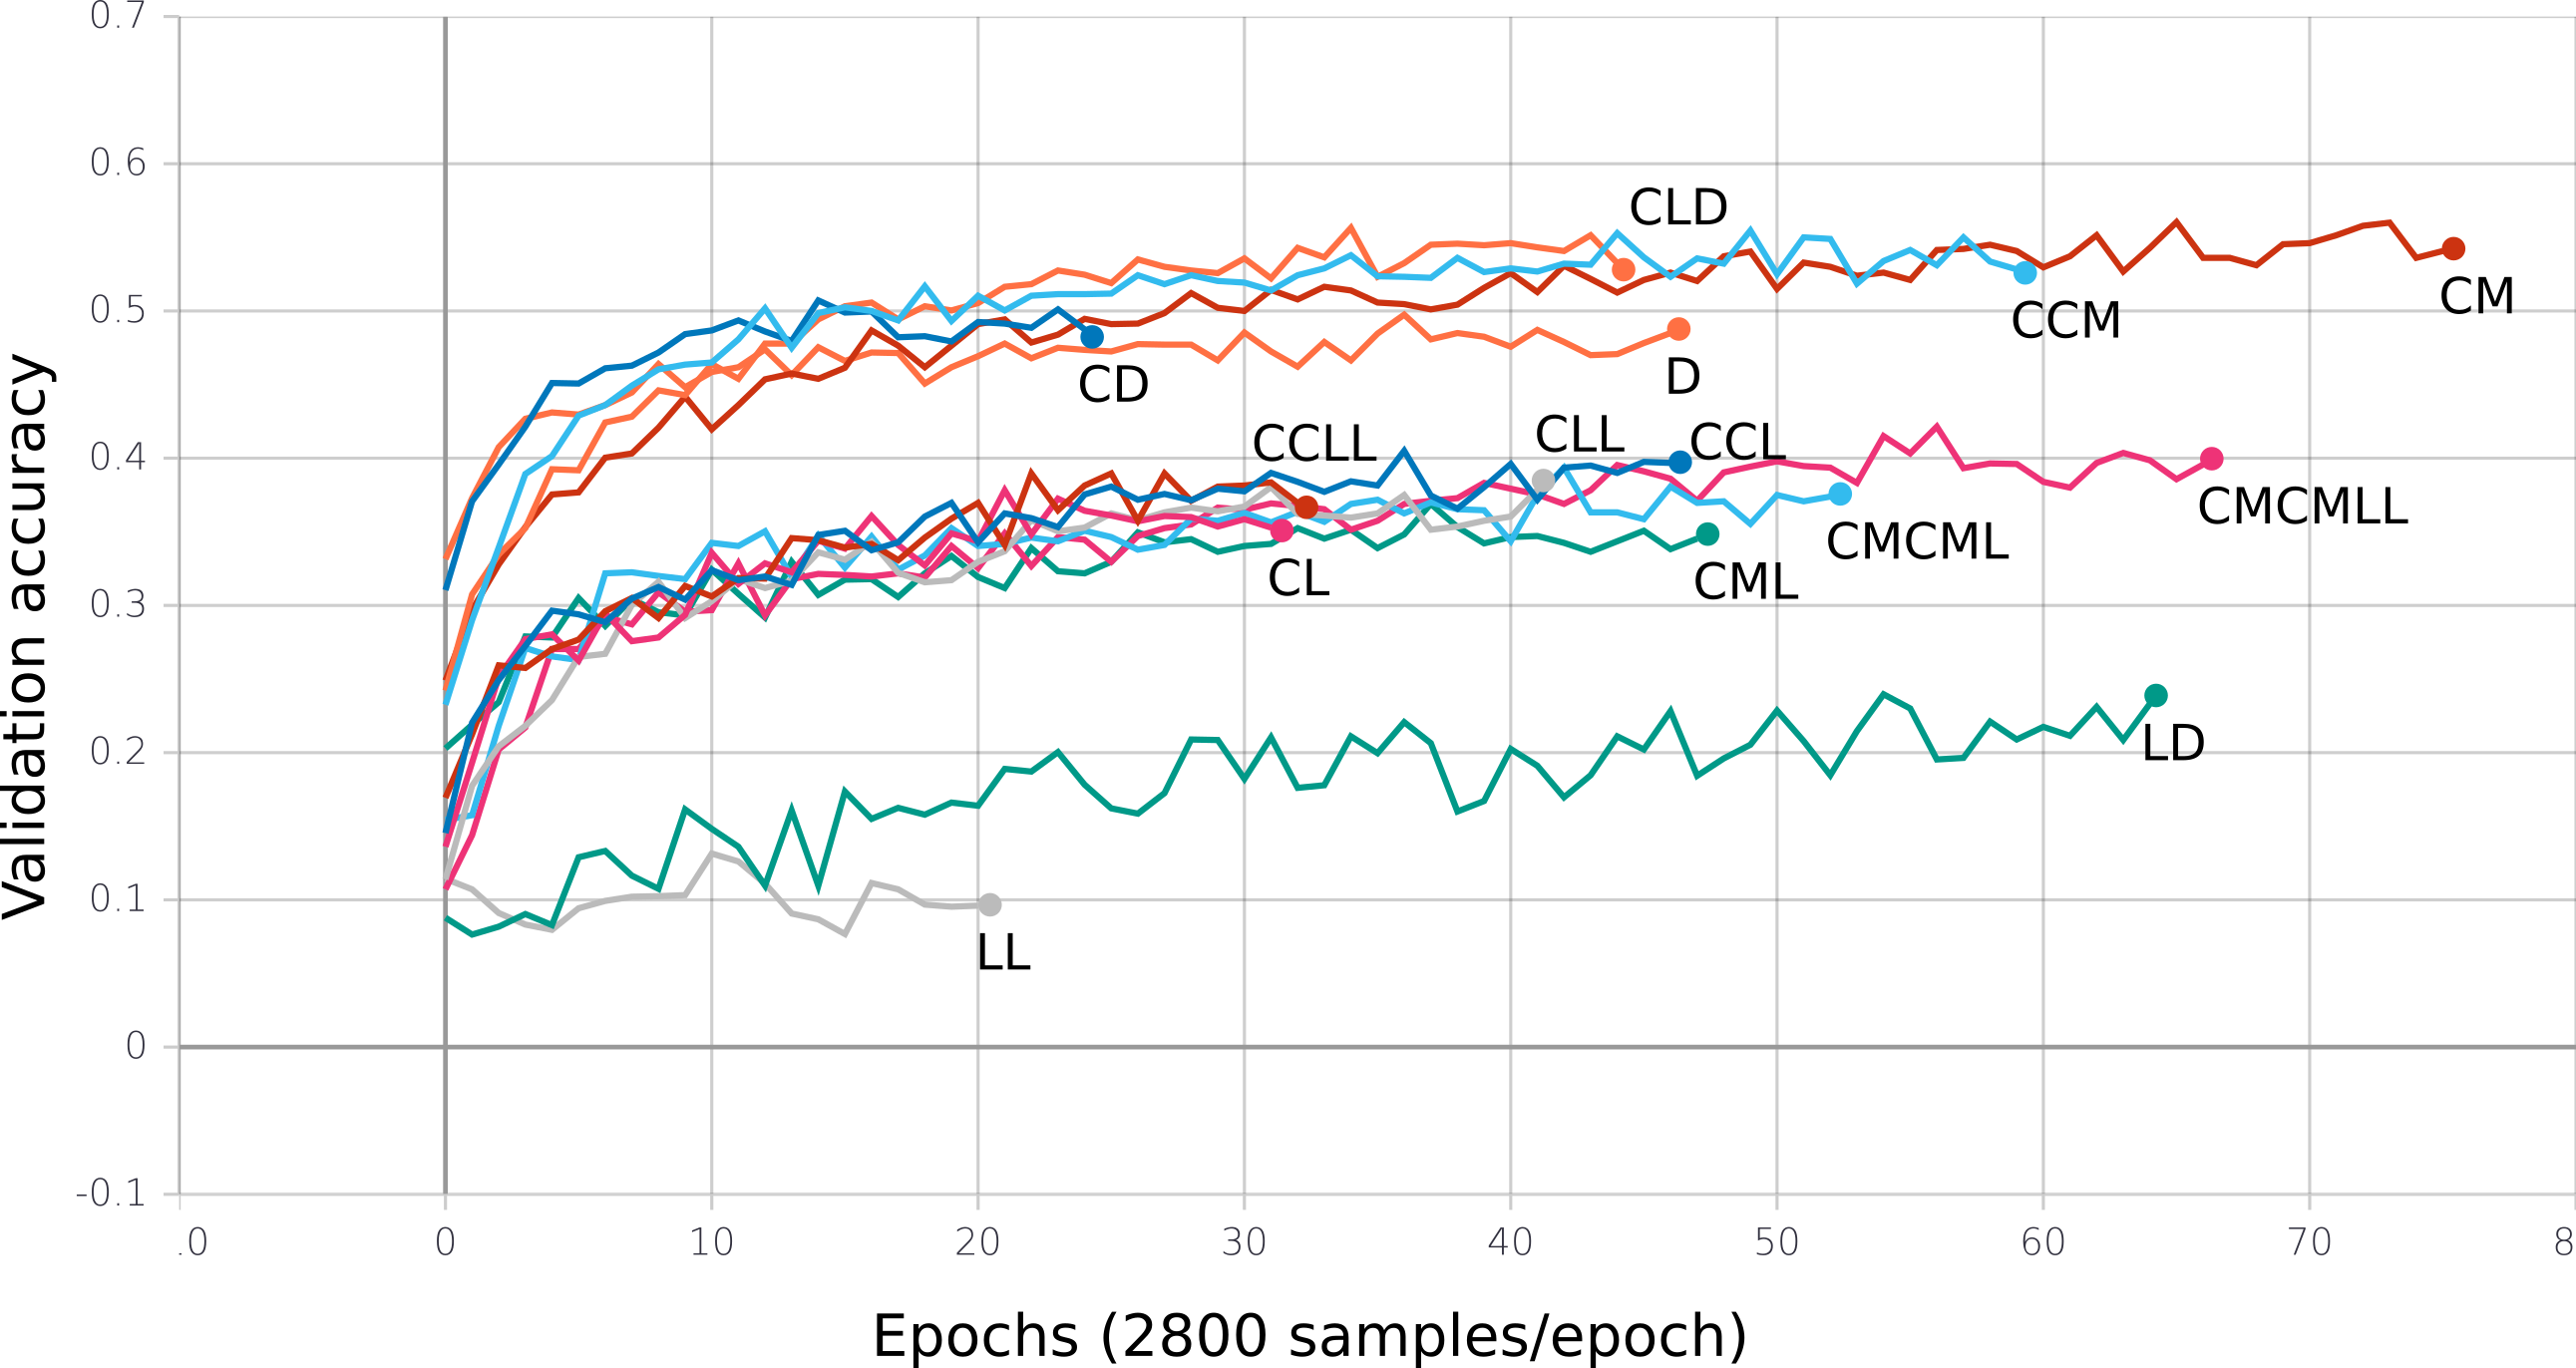
\includegraphics[width=0.9\textwidth]{content/epoch_val_categorical_accuracy.png}
\caption{\label{fig:learning}Learning curves of some models (validation accuracy vs. time)}%
\end{figure*}

%\levelB{Inputs}
%one-hot
The input features of the network for each instance is a 512x256 matrix representing only one block of 512 bytes of a random file of the dataset. Each of the 512 bytes is one-hot encoded, meaning that its value is converted into a vector with 256 elements, with only one of them set to 1, corresponding to the value of the byte, while the others are set to zero. A batch size of 100 was used, with 28 steps per epoch.

%8bits
% The input features of the network for each instance is a 512x8 matrix representing only one block of 512 bytes of a random file of the dataset. Each of the 512 bytes uses a custom encoding where each of the 8 bits of a byte is represented as -1 or 1, depending whether the bit is 0 or 1. During initial tests, this encoding was compared to three other encodings: one-hot encoding, 8 bits represented as 0 or 1\todo{include citation}, and 8 bits represented as [0,1] and [1,0] \cite{hiester_file_2018}. More research should be done in the future to determine the best of the four, but initial results suggest they have similar impact on the model accuracy. The one-hot encoding has the disadvantage of increasing the input matrix size by a factor of 32.

%\levelB{Outputs}
The output of the network for a given instance is a vector with a size equal to the number of classes, subjected to a softmax function, which applies the exponential function on the vector and then normalizes it. Each value will represent the predicted probability that the instance belongs to a specific class.

%exp18
The two models that used LSTM layers without convolutional layers presented slower learning in comparison with the others, as can be seen in figure \ref{fig:learning}. The final validation accuracy values can be consulted in figure \ref{fig:models}.


\noindent
\begin{figure*}[htb!]
\centering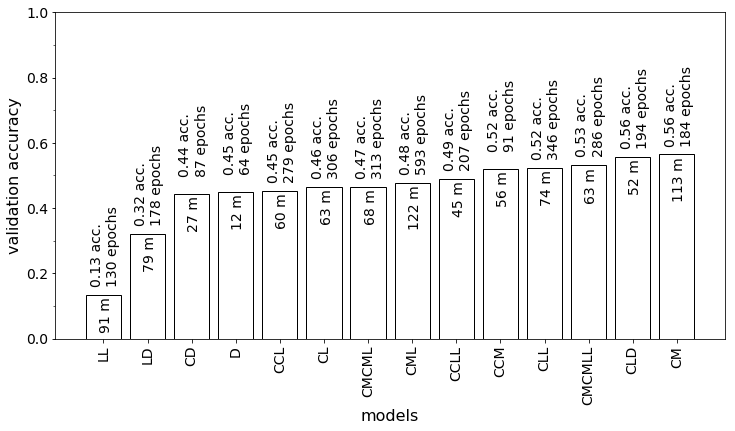
\includegraphics[width=1.0\textwidth]{content/models.png}
\caption{\label{fig:models}The bar plot shows the validation accuracy of the considered models. Their training time, in minutes, and the total epochs processed is also indicated. The training was interrupted when no further improvement was observed for 10 consecutive epochs.}%
\end{figure*}


The validation accuracy values of the remaining models were in the 0.35-0.54 range.

% The selected model for further research, identified as ``CM'', achieved an accuracy of 0.54. The models, ``CLD'' and ``CCM'' achieved similar values, but model ``CM'' performed better in the experiment described in section \ref{sec:exprandom}.

To check if the two slower models could give better results if executed for a longer period, they were trained for 10 hours. The model identified as ``LD'', which uses an LSTM layer followed by a fully connected layer, was able to achieve an accuracy of 0.494, while the other, ``LL'', achieved only 0.153.

%stagnation in learning with such short times, combined with low final accuracy suggests that the dataset present some patterns that are easily recognizable, while the rest of the dataset present a very hard classification task.

% \levelC{Limitations and threats to validity}

The model CLD was chosen to be compared with other works because it was among the 3 models with highest accuracy, but achieved its results in less time and showed high resilience to changes in parameters during the tests, while the others did not.
 
In this second stage, using longer training sessions, the accuracy for the 28 file types used in the first stage increased from 0.54 to 0.63. Using the same file types of other works, the CLD model achieved an accuracy of 
0.67 for the file types from Chen \textit{et al.} \cite{chen_file_2018},
0.91 for Hiester \cite{hiester_file_2018}, 
0.59 for Wang \textit{et al.} \cite{wang_sparse_2018},
0.65 for Wang \textit{et al.} \cite{wang_file_2018},
and
0.61 for Vulinović \textit{et al.} \cite{vulinovic_neural_2019}.
The results can be seen in figure \ref{fig:cldothers}.

\noindent
\begin{figure*}[htb!]
\centering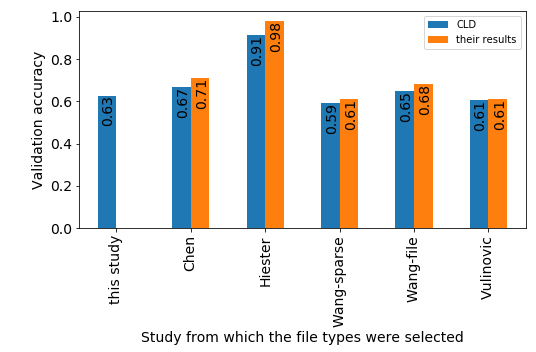
\includegraphics[width=0.8\textwidth]{content/CLD-others.png}
\caption[CLD vs. other studies]{\label{fig:cldothers}The CLD model was trained from scratch using the same file types used in other works. The bar plot shows the comparison between the validation accuracy obtained with CLD and those achieved in other studies.}%
\end{figure*}

    \levelB{Discussion}
    This chapter presented some alternative models in the file fragment classification task. The idea was to identify the most promising models for improvement. But an apparent limit was found on how far these models could be improved.

Answering the first research question ``\textbf{How do different neural network models compare to each other in terms of training performance and quality of results in file fragment classification?}'', 
the results may be grouped into three sets: i) the models that used LSTM without a convolutional layer performed poorly; ii) the models with convolutional layers that used LSTM as the last layer had intermediary results; iii) the remaining models, which achieved better results, were the single-layer perceptron (single fully-connected layer model, identified as ``D'') and the models that used convolutional models and used a fully-connected layer or max pooling as the last layer.

The three models with best accuracy results are identified as ``CCM'', ``CM'', and ``CLD'', but the latter had faster training time and also showed good resilience to changes: during preliminary tests and later when test conditions were altered to try to improve results, this model and its variations were always among the best models.

In this stage of the research, the models were not trained to exhaustion.
This was initially done to identify which models would be most promising for future testing, but further attempts to tune layer types, quantity and parameters resulted in accuracy values still close to 60\%.
Most models required short training times and few examples to approach their limits.
This suggests that some patterns were very easy to find but they were insufficient to achieve higher accuracy.
This raises the question of whether there are harder patterns that could be found by a better model not yet tried or if this a more fundamental issue that would not be solved by a trial and error approach of tweaking of parameters and layer modifications.

However, the 14 models used in this study represent a very small sample of all possible model architectures using the chosen layer types. Moreover, there is no certainty that in different circumstances the best performing models will continue to outperform the others. For those reasons, the search for an alternative model could also be a valid research direction. Since the proposed models use a small number of layers and considering that deep networks have shown good results in other applications, a study that increases the number of layers of the models presented here may improve results.

A comparison was made between a chosen model, ``CLD'', and recent works in the field. While ``CLD'' achieved slight lower accuracy values than the other studies, it can be noticed that the values are similar:
while the result values of these other works range from 61\% to 98\%, a difference of 37\%, the differences between the results from this study and theirs do not exceed 7\%. This is an indication that the high  variability that these studies show between each other is caused by the difference in the file types they choose. This supports the claim that advances in this area should come from error analysis.

The Govdocs1 dataset brought an important basis for comparison to be used between carving solutions. But to achieve easily reproducible results, the models must also be publicly available, a condition not all revised studies fulfill. Being available as Jupyter notebooks at https://github.com/atilaromero/carving-experiments, the results described here should require little effort to be reproduced. Thus the source code can be used as a basis of comparison in future researches, generating models with the same architecture of those presented here.


%5
\levelA{Descriptive research on influence of number of classes}
\label{sec:numberofclasses}
    % \levelB{Objective}
In Chapter \ref{sec:evalmodels}, it was observed that achieving accuracy values above 60\% on file fragment classification using 28 classes was a difficult task to the considered models. In other studies results \cite{hiester_file_2018} \cite{sportiello_context-based_2012} \cite{amirani_feature-based_2013} \cite{maslim_distributed_2014} and on initial tests, the achieved accuracy for a small number of classes was considerably higher. Hiester \cite{hiester_file_2018}, for instance, achieves an accuracy of 98\% using four classes.

To address the second research question 
``\textbf{How does the accuracy of neural network models changes relative to the number of classes?}'', 
this chapter describes several neural network training sessions using different sets of file types and the attempt to understand how the accuracy of the resulting models are affected by composition of file types in the set.


    \levelB{Method}
    \todo[inline]{include method figure}

\todo[inline]{refer to chapter 4}
% \levelB{Dataset}
This study uses the Govdocs1 dataset \cite{garfinkel_bringing_2009}, which was fully downloaded and its files were grouped by extension. This dataset has files with 63 different extensions. The 33 extensions with less than 200 files were discarded. The  ``text'' and ``unk'' extensions were discarded because files with these extensions use multiple formats and they do not correspond to a single file type. From the remaining 28 extensions, listed in table \ref{tab:studiesfiletypes}, 200 files of each were randomly selected, 100 to use in the training dataset and 100 to use in the validation dataset.

% \begin{table}[!ht]
    \centering
    \caption{Govdocs1 dataset}
    \label{tab:govdocs1}
\begin{tabular}{|l|l|l|}
\hline
Extension & Number of files & Number of blocks \\ \hline
                                                  \hline
pdf       & 231232          & 268071071    \\ \hline
html      & 214568          & 25710908     \\ \hline
jpg       & 109233          & 73242253     \\ \hline
txt       & 78286           & 99435540     \\ \hline
doc       & 76616           & 60654930     \\ \hline
xls       & 62635           & 58718224     \\ \hline
ppt       & 49702           & 251210471    \\ \hline
gif       & 36302           & 5962516      \\ \hline
xml       & 33458           & 16954875     \\ \hline
ps        & 22015           & 56547464     \\ \hline
csv       & 18360           & 6843009      \\ \hline
gz        & 13725           & 17748905     \\ \hline
log       & 9976            & 8467819      \\ \hline
eps       & 5191            & 5756138      \\ \hline
% unk       & 5186            & 2983922      \\ \hline
png       & 4125            & 2207489      \\ \hline
swf       & 3476            & 3798321      \\ \hline
dbase3    & 2601            & 38972        \\ \hline
pps       & 1619            & 7432480      \\ \hline
rtf       & 1125            & 958239       \\ \hline
kml       & 993             & 309422       \\ \hline
kmz       & 943             & 549462       \\ \hline
% text      & 839             & 1527118      \\ \hline
hlp       & 659             & 8692         \\ \hline
f         & 602             & 94543        \\ \hline
sql       & 462             & 244634       \\ \hline
wp        & 364             & 87643        \\ \hline
dwf       & 299             & 85500        \\ \hline
java      & 292             & 14530        \\ \hline
pptx      & 215             & 1151796      \\ \hline
% fits      & 182             & 678128       \\ \hline
% tmp       & 180             & 28426        \\ \hline
% tex       & 163             & 10520        \\ \hline
% docx      & 163             & 65969        \\ \hline
% troff     & 110             & 8020         \\ \hline
% bmp       & 72              & 62686        \\ \hline
% sgml      & 62              & 44138        \\ \hline
% gls       & 60              & 517          \\ \hline
% pub       & 55              & 1421         \\ \hline
% xlsx      & 37              & 12910        \\ \hline
% fm        & 25              & 6717         \\ \hline
% zip       & 10              & 31525        \\ \hline
% ttf       & 10              & 1540         \\ \hline
% xbm       & 8               & 578          \\ \hline
% wk1       & 7               & 6493         \\ \hline
% sys       & 7               & 15           \\ \hline
% ileaf     & 4               & 1656         \\ \hline
% exported  & 3               & 324          \\ \hline
% data      & 3               & 1733         \\ \hline
% odp       & 2               & 2384         \\ \hline
% mac       & 2               & 0            \\ \hline
% lnk       & 2               & 2            \\ \hline
% js        & 2               & 36           \\ \hline
% g3        & 2               & 498          \\ \hline
% chp       & 2               & 73           \\ \hline
% 123       & 2               & 434          \\ \hline
% wk3       & 1               & 229          \\ \hline
% vrml      & 1               & 660          \\ \hline
% squeak    & 1               & 25354        \\ \hline
% py        & 1               & 480          \\ \hline
% pst       & 1               & 20           \\ \hline
% icns      & 1               & 0            \\ \hline
% bin       & 1               & 7            \\ \hline
\end{tabular}
\end{table}


% \levelB{Sampling}
To select a sample instance from the Govdocs1 dataset, first, a random file is selected among those available, without replacement. Then, a block from this file is randomly selected. After all files have participated in the process, it may be repeated as many times as necessary. This way, all files are considered, and the classes are easily balanced.
This contrasts with the sampling technique applied in other works, where all the sectors are grouped before sampling, which may lead to an imbalance between classes.

% \levelB{Inputs}
%one-hot
The input features of the network for each instance is a 512x256 matrix representing only one block of 512 bytes of a random file of the dataset. Each of the 512 bytes is one-hot encoded, meaning that its value is converted into a vector with 256 elements, with only one of them set to 1, corresponding to the value of the byte, while the others are set to zero. A batch size of 100 was used, with 28 steps per epoch.

% \levelB{Outputs}
The output of the network for a given instance is a vector with a size equal to the number of classes, subject to a softmax function, which applies the exponential function on the vector and then normalizes it. Each value will represent the predicted probability that the instance belongs to a specific class. The class for a block sample is the file extension of the original file.

% \levelB{Model}
The model architecture used in this research, ``CLD'', is described in the previous chapter and has three layers. The first is a convolutional layer with 256 output units, a window of size 16, and a stride of 16. The second is an LSTM layer of 128 units. The last is a fully-connected layer where the number of output units matches the number of classes of the input dataset.

%optimization
All the training sessions used the Adam \cite{kingma_adam:_2014}
optimization algorithm to guide backpropagation, which was selected because it performed well in the preliminary tests without requiring fine-tuning of parameters.

% Constraints
The models were trained until no further improvement was observed in the last 10 epochs, using categorical cross-entropy loss.

\levelC{Accuracy vs. number of classes}
Several independent models with the same general architecture, but different weights, were trained with 2 to 28 extensions from the Govdocs1 dataset. For each number in the range 2 to 28, a random subset of extensions was selected to compose the dataset. Each extension has 200 file samples, half placed in the training dataset and half in the validation dataset. Each dataset was used to train a new model, that should distinguish between the selected subsets of extensions in that filtered dataset. This process was repeated five times.

In addition to this sampling of extensions using different quantities of classes, all 378 combinations of pairs of extensions were compared. Each pair was used to compose a dataset and to train a new model for each one, using the same process described in the previous paragraph.

Given the number of different models trained (135 for the N classes phase and 378 for the pairs), it was important to use a model architecture that had a fast training time. Models trained with the chosen architecture took about 10 minutes to train. Without this short training period, this research would not be feasible.

\levelC{PCA}
The accuracy obtained after the training of models with pairs of classes was used to build a 28x28 matrix. Here the accuracy of the model trained for that particular pair of extensions was used as a distance measure of how similar those file types are. If a model was able to achieve 100\% accuracy, the file types would be considered different, if the accuracy is 50\%, they would be considered indistinguishable, as 50\% is the average accuracy of a random guess classifier for two classes.

Following this concept, the diagonal entries of the matrix were filled with the value 0.5, as each class should be indistinguishable from itself. Then, a Principal Component Analysis (PCA) \cite{amirani_new_2008} was used to treat this matrix. The 28x28 matrix can be interpreted as 28 vectors of 28 dimensions. For each class, the vector indicates how similar that class is to each of the others. This could be plotted in a space of 28 dimensions if such representation could be built. What PCA does is to reduce the dimensionality of this space. Here the dimensions were reduced to two, to be shown in a 2D graph. To do that, it chooses as first axis the one that maximizes the variance in the data and then does the same for the second dimension. That produces a projection in which the points are as farther away as possible.

While it may not be obvious how to attribute meaning to the resulting coordinate system, this technique is useful to visually group classes with similar characteristics.



    \levelB{Results}
    % \levelB{Hardware}
The experiments did not take advantage of GPU acceleration and were  conducted on a single computer with 256GB of RAM and with 2 Intel\textregistered Xeon\textregistered E5-2630 v2 processors, with 6 cores each, with 2 hyper-threads per core, or 24 hyper-threads in total. 


% \levelB{Software}
The main software and frameworks used to build the experiments were Python 3.6 \cite{rossum_python_2019}, Jupyter notebook \cite{perez_jupyter_2019}, Tensorflow 1.14.0 \cite{google_brain_tensorflow_2019}, Keras 2.2.4-tf \cite{chollet_keras_2019}, and Fedora Linux 27.
% repository
The source code for the experiments is available at \sloppy\url{http://github.com/atilaromero/carving-experiments}.

\levelC{Accuracy vs. number of classes}

% decrease in accuracy
Figure \ref{fig:nclasses} shows the graph of accuracy versus number of classes.  Each of those points is a model trained with the indicated number of classes. The class for a block sample is the file extension of the original file. The classes/extensions used to train each model were taken at random. The bottom line indicates for comparison how accurate a random guess classifier would be. The points for two classes use transparency to improve visualization, as many of them are too close. For 2 classes, the accuracy values are between 50\% and 100\%, with a greater concentration near 100\%. For 28 classes, the accuracy values are between 55\% and 58\%.

The lines ``hard file types first'' and ``easy file types first'' were created by selecting the file types that would compose the dataset. The selection was based on the results described in the next subsection, ``Accuracy of pairs of classes'', ordering the file types by their minimum accuracy values and following this order to choose file types. For example, the ``hard file types first'' point for three classes was obtained by training a model with the file types ``pps'', ``ppt'', and ``gz'', the three classes with lower minima in Figure \ref{fig:dual}.

\noindent
\begin{figure*}[htb!]
\centering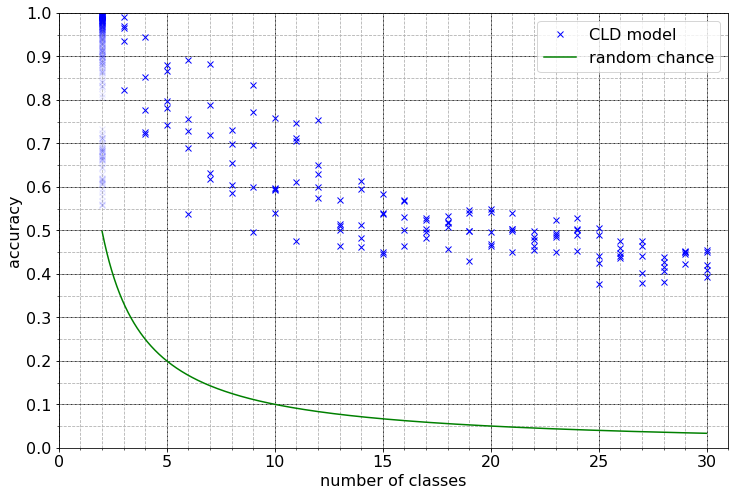
\includegraphics[width=0.8\textwidth]{content/nclasses.png}
\caption{\label{fig:nclasses}Validation accuracy by number of classes}%
\end{figure*}

\levelC{Accuracy of pairs of classes}

Figure \ref{fig:dual} shows the graph of the accuracy of each class when compared individually with each one of the others, resulting in 378 models, one for each possible pair of classes. File types where all the points are close to 100\% are hardly mistaken for other types, while file types presenting accuracy values close to 50\% can be mistaken for other file types by the model.

\noindent
\begin{figure*}[htb!]
\centering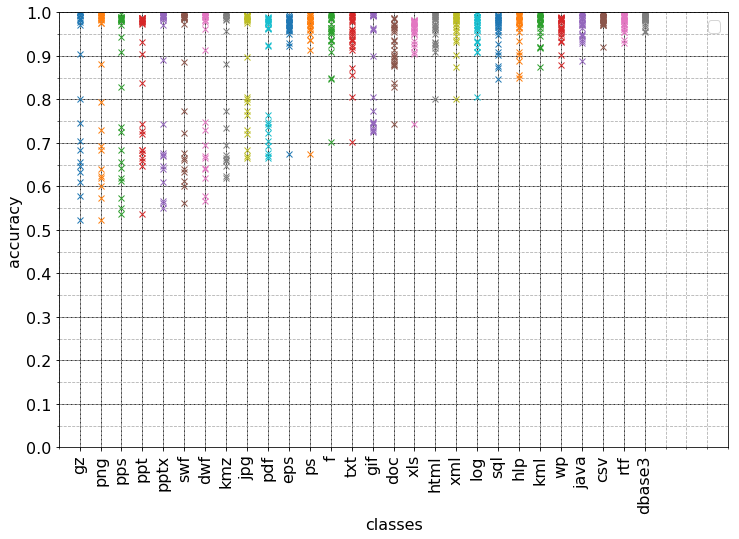
\includegraphics[width=0.8\textwidth]{content/dual.png}
\caption{\label{fig:dual}Validation accuracy of models trained with pair of classes}%
\end{figure*}

\levelC{PCA}

A 28x28 matrix was made using the accuracy of the models built for each pair of classes as a distance measure. A PCA dimensionality reduction technique was used to plot this data in a 2D graph, grouping similar file types. The result is shown in figures \ref{fig:pca} and \ref{fig:pca2}. Similar file types are next to each other, while those that can be easily distinguished by the models are represented by points that are distant from each other.

\noindent
\begin{figure*}[htb!]
\centering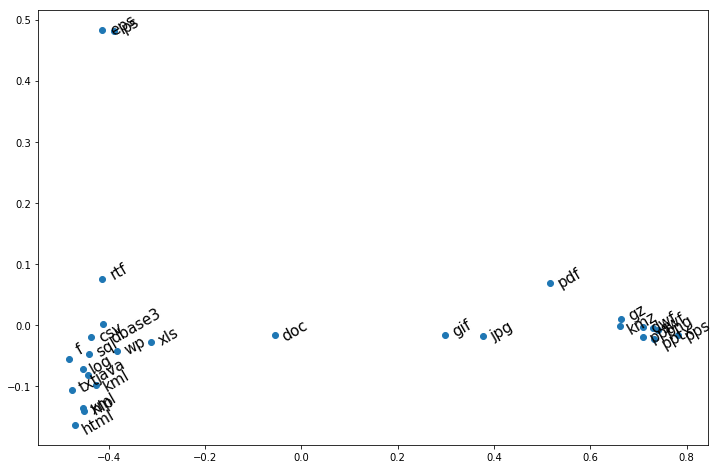
\includegraphics[width=0.8\textwidth]{content/pca.png}
\caption{\label{fig:pca}PCA of accuracy of models trained with pair of classes}%
\end{figure*}


\noindent
\begin{figure*}[htb!]
\centering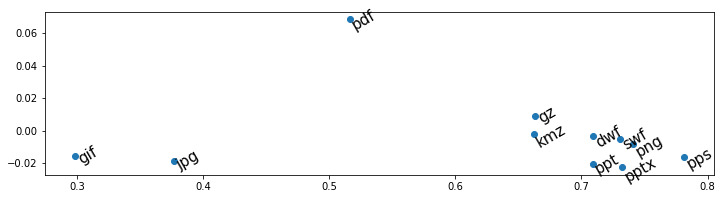
\includegraphics[width=0.8\textwidth]{content/pca2.png}
\caption[PCA of accuracy of models trained with pair of classes - detail]{\label{fig:pca2}PCA of accuracy of models trained with pair of classes - lower right detail}%
\end{figure*}

% the problem of unseen file types
% \levelC{Limitations and threats to validity}


    \levelB{Discussion}
    
%fig 1
\levelC{Accuracy vs. number of classes}

In figure \ref{fig:nclasses}, a decreasing trend was observed. An increase in the number of classes appears to be  correlated with a decrease in accuracy. Another relevant aspect of the graph is that the range of the results seems to be smaller when more classes are used.  

This pattern is understandable: as the number of classes grows, the harder the classification problem is, leading to a decrease in accuracy. Meanwhile, the individual contributions of each class to the overall result diminishes, leading to an increase in precision.

This behavior is an important aspect to consider during the evaluation of file fragments studies. This observation is in agreement with Beebe et al. \cite{beebe_sceadan:_2013} observation, that studies that select fewer classes tend to yield higher results. 

Still, with 42\% \footnote{In the extended training session described in chapter 4, a higher accuracy was obtained and 38\% of samples were misclassified, instead of 42\%.} of samples being misclassified when the number of classes is 28, the question of what are the error sources and how they can be addressed requires attention.

The number of possible combinations of file types to compose the datasets depends on the number of classes being considered. For 28 classes there is only one possible combination, while for two classes there are 378. For intermediary values, the numbers are much higher, which is the number of possible combinations disregarding the order of the elements: $ \frac{28!}{(28-n)!n!}$. For 14 file types there are 40116600 combinations. For this reason, the significance of the 5 samples diminishes for intermediary values.

\levelC{Accuracy of pairs of classes}

The accuracy of models trained with pairs of classes, shown in figure \ref{fig:dual}, suggests a reverse correlation between entropy and accuracy.  Generally, file types with higher entropy tend to have lower minima, with the GIF file type being a notable exception. Most of these files use some form of compression, like image files for example.

It was demonstrated that the accuracy of a new model may be manipulated by the selection of file types that will compose the dataset. The lines ``hard file types first'' and ``easy file types first'' of figure \ref{fig:nclasses} were created using the order shown on figure \ref{fig:dual}, resulting in lines that seem to be close to the minimum and maximum of the possible accuracy values. 

\levelC{PCA}

The usage of PCA on the 28x28 distance matrix produced a 2D projection where, as shown in figures \ref{fig:pca} and \ref{fig:pca2}, a group of file types that use compression or contains images are grouped near each other: 
``gif'',
``jpg'',
``pdf'',
``gz'',
``kmz'',
``dwf'',
``ppt'',
``swf'',
``png'',
``pptx'',
and ``pps''.

\levelC{Conclusion}
It was observed that an increase in the number of extensions selected to compose the training has the tendency to decrease accuracy and increase precision. But the number of classes alone is not as important as the type of extension selected: some file types when included in the experiment have a much higher negative impact than others. This observation was demonstrated in the ``hard file types first'' and ``easy file types first'' of figure \ref{fig:nclasses}, where the file types selected to compose  where intentionally chosen, once to degrade results and once to improve them.

File types that contains images or that use compression were identified as those that have the higher negative effect on results, which suggests that their entropy may contribute to the error.

% \levelB{Limitations, threats to validity and future work}

The number of samples taken was small when compared with the number of all possible file types combinations. This imposes a limit on the conclusions that can be reached and this limitation is hard to overcome.

The group that emerged as file types that most degrade results are files that use compression or contain images. While they are known for their high entropy, no measure of entropy was used to reinforce this claim.
This aspect is addressed in the next chapter.
% A study is in progress to measure the impact of entropy on file fragment classification errors.

%6
\levelA{Experiment on random data detection}
\label{sec:exprandom}
    % \levelC{Objective}
In the previous chapter, it was observed that file types that use compression or contain images have a higher negative impact on accuracy than other file types do. This raises the question of whether high entropy may be related to the observed errors.

Before conducting experiments related to the cause of errors, a list of conceivable error sources (E1 to E5) was elaborated:
\begin{enumerate}[itemindent=\parindent,label=\textbf{E\arabic*.}]
    \item For some data structure, the model cannot distinguish it from random data. This can happen if the pattern in the data is too complex, beyond the capabilities of the model. It may be the case that in practice no model can perform this distinction or, instead, this may be a limitation of this particular model only. This situation may occur in files that use compression or cryptography, or more generally, any file type with high entropy.
    
    \item Different file types using different data structures, but the model cannot distinguish between them. In this case, the model can perceive that there are structures in the data, but it is not able to differentiate them.

    \item Different file types using the same data structure. It is common for a given file type to employ different types of data structures. If two or more file types make use of the same data structure, the existence of that structure will then not be sufficient to differentiate those file types, as it may belong to any of them.
    The reverse, a file type that uses multiple kinds of data structures, does not constitute a problem as it simply results in extra work during the model training.

    \item Same file type with multiple extensions. If the same file type appears in the dataset with multiple extensions, ``JPG'' and ``JPEG'' for example, the model will not be able to predict which label is used in the validation dataset for a given instance, since this distinction exists in the labeling, but not in the content.

    \item Files that contain other files. Some file types need to embed other files. If the inner file is categorized, even if the model finds an unmistakable pattern, it will not match the label, which will be the extension of the outer file. A ``PDF'' file, for example, can embed a ``JPG'' file. If the model predicts ``JPG'' as the class of a portion of this file, it will not match the instance label on the dataset, which would be ``PDF''.
\end{enumerate}

The first error source, E1, is the focus of this chapter. In the file fragment classification task, it is expected that some portion of the classification errors of a given model be caused by its inability to recognize patterns in the data if the data have high entropy. In these situations, even humans may be unable to tell if a sample is valid or if it is random data. A search for an alternative model may lead to better results, but the chances are low, as this type of error is hard to mitigate. 

In the second error source, E2, it is conceivable that avoiding misinterpretation of one structure as another is possible since the model has successfully detected structures. This error source is not explored in this study. Mitigation of this type of error probably would be achieved through more training or by a search for a better model.

The three last error sources listed above, E3 to E5, are not explored in this study. They are similar in nature, as the last two may be viewed as special cases of E3. This type of error is best mitigated through a revision of the labeling system.

\todo[inline]{include research question}

% \levelC{Hypothesis}
The goal of the experiment of this chapter is to test the \textbf{hypothesis that part of the errors of file fragment classification can be explained by the inability of the models to distinguish high entropy data from random data}. Not all file types have this kind of data, and for those that do, they should compose only a portion of the file.

% Two methods are described next. The measuring method results in a number that can be used as a measure of entropy. The filtering method can be used to filter the original dataset, leaving only samples that have recognizable structures.


    \levelB{Method}
    \todo[inline]{include method figure}

% \levelC{Models}
For this experiment, a new model is created for each considered file type. The input of the model is a one-hot encoded block than may come from a random generator or from the Govdocs1 dataset. Samples from the Govdocs1 dataset are labeled ``structured'', while samples from the random generator are labeled ``random''. The model should predict from which source the sample came.

The 28 file types from the Govdocs1 dataset \cite{garfinkel_bringing_2009} used in chapters \ref{sec:evalmodels} and \ref{sec:numberofclasses} were used in this experiment, placing 100 files in the training dataset and 100 in the validation dataset.


The model architecture used in this research stage, ``CLD'', is described in Chapter \ref{sec:evalmodels} and has three layers. The first is a convolutional layer with 256 output units, a window of size 16, and a stride of 16. The second is an LSTM layer of 128 units. The last is a fully-connected layer where the number of output units matches the number of classes of the input dataset.

All the training sessions used the Adam \cite{kingma_adam:_2014}
optimization algorithm to guide backpropagation.
The stopping condition used is 10 epochs without improvement in validation accuracy, using categorical cross-entropy loss.


\levelC{From data source to measure of entropy}
There is a difference in the nature of the predetermined labels and the predicted ones. The predetermined labels reflect the data source from which the samples were extracted, while the predicted labels are based on the content of the data. For the random generator, this is not a problem, as this data source only has one kind of data. But the samples from the Govdocs1 dataset may have two kinds of data. For some of the samples, it is expected that the true classification should be ``random'' instead of ``structured''. These are the samples that are too complex to this kind of model, the ones where the model cannot find any pattern. Unfortunately, there is no direct way to know the perfect labels in advance, hence all samples of the Govdocs1 dataset are labeled ``structured''. Thus, it is known that the samples from Govdocs1 dataset have an unknown portion of conditions positives and negatives.

Here, the ``structured'' samples are considered positive and the ``random'' samples are considered negative. Thus the samples that are classified as ``random'' by the model are the sum of the true negatives and the false negatives. Similarly, the samples classified as ``structured'' are the sum of the true positives and the false positives.

The random generator can be used to predict the proportion between false positives and true negatives of the chosen file type from the Govdocs1 dataset. Since the condition negative (which is the sum of false positives and true negatives) is those samples that ideally should be marked ``random'', the classifier should treat them the same way it treats the random generator samples.

In other words, the Govdocs1 dataset for a particular file type is assumed to have a subset of samples that should be labeled ``random'' because the model cannot find patterns in them. Some of those samples may be incorrectly labeled ``structured'' by the model. These are the false positives. But this should happen in the same proportion that the model classifies samples from the random generator as ``structured''.

Using this method, the quantity that would best represent the entropy of the dataset would be $(1-Prevalence)$, where  $Prevalence=\frac{\sum ConditionPositive}{\sum TotalPopulation}$. Unfortunately, without knowing the false negative rate, the best that can be achieved is a range where the maximum entropy value occurs when the false negative rate is zero. Assuming the false negative rate to be zero, the prevalence will be equal to the true positives over the entire population. Thus, the entropy range can be calculated using only the accuracy values of the trained model obtained separately on the Govdocs1 dataset and on the random dataset, as shown in equations \ref{eq:TPstart} to \ref{eq:TPend}.

\begin{align}
\label{eq:TPstart}
    1-\begin{matrix}
    Entropy\\
    measure
    \end{matrix}
      &= Govdocs\,True\,Positive \\
      &= Govdocs\,Predicted\,Positive - Govdocs\,False\,Positive\\
      &= GovdocsPredPOS - \left(GovdocsPredNEG*\frac{randomPredPOS}{randomPredNEG}\right)\label{eq:TPPred}\\
      &= GovdocsKerasACC - \frac{(1-GovdocsKerasACC)*(1-randomKerasACC)}{randomKerasACC}
      \label{eq:TPend}
\end{align}

In equation \ref{eq:TPPred}, the $(GovdocsPredNEG)$ quantity is the portion of samples marked as ``random'' by the model when classifying samples from the Govdocs1 dataset. Normally, $Predicted\,Negative = True\,Negative + False\, Negative$, but the no false negative assumption is being used. The $GovdocsKerasACC$ is the accuracy calculated by Keras during validation of the Govdocs1 dataset. It is not the real accuracy since this validation considers all samples marked ``random'' as errors. Thus $GovdocsKerasACC = GovdocsPredPOS$. The accuracy calculated by Keras during validation of the random generator consider as correct the samples marked as ``random'', thus $randomKerasACC = randomPredNEG$.

Multiplying $(1-GovdocsKerasACC)$ value by $\frac{(1-randomKerasACC)}{randomKerasACC}$ should give the portion of samples that are erroneously marked as ``structured'' by the model, the false positives. Here it is assumed that $\frac{False\, positive}{True\,negative}$ on the Govdocs dataset is equal to $\frac{randomPredPOS}{randomPredNEG}$ on the random generator.

After this entropy measure is calculated for all the file types, it can be used to estimate the amount of error that can be attributed to the model's inability to recognize structures, testing the proposed hypothesis. For a dataset with a balanced file type distribution, this will be the mean of the entropy measures.


    % \levelB{Filtering method}
    % This section describes an alternative to the method presented in the previous section. Instead of calculating the proportion of true positives in the population, the samples of the Govdocs1 dataset that are labeled ``structured'' are used as input to train a second model, that will be used to validate the first model.

% \levelC{Dataset}
The model training was divided into two passes, depicted in Figure \ref{fig:randommeasure}. Each pass trains a different model for each file type. In the first pass, the dataset creation of a given file type follows the same procedure mentioned in the previous section.

\noindent
\begin{figure*}[htb!]
\centering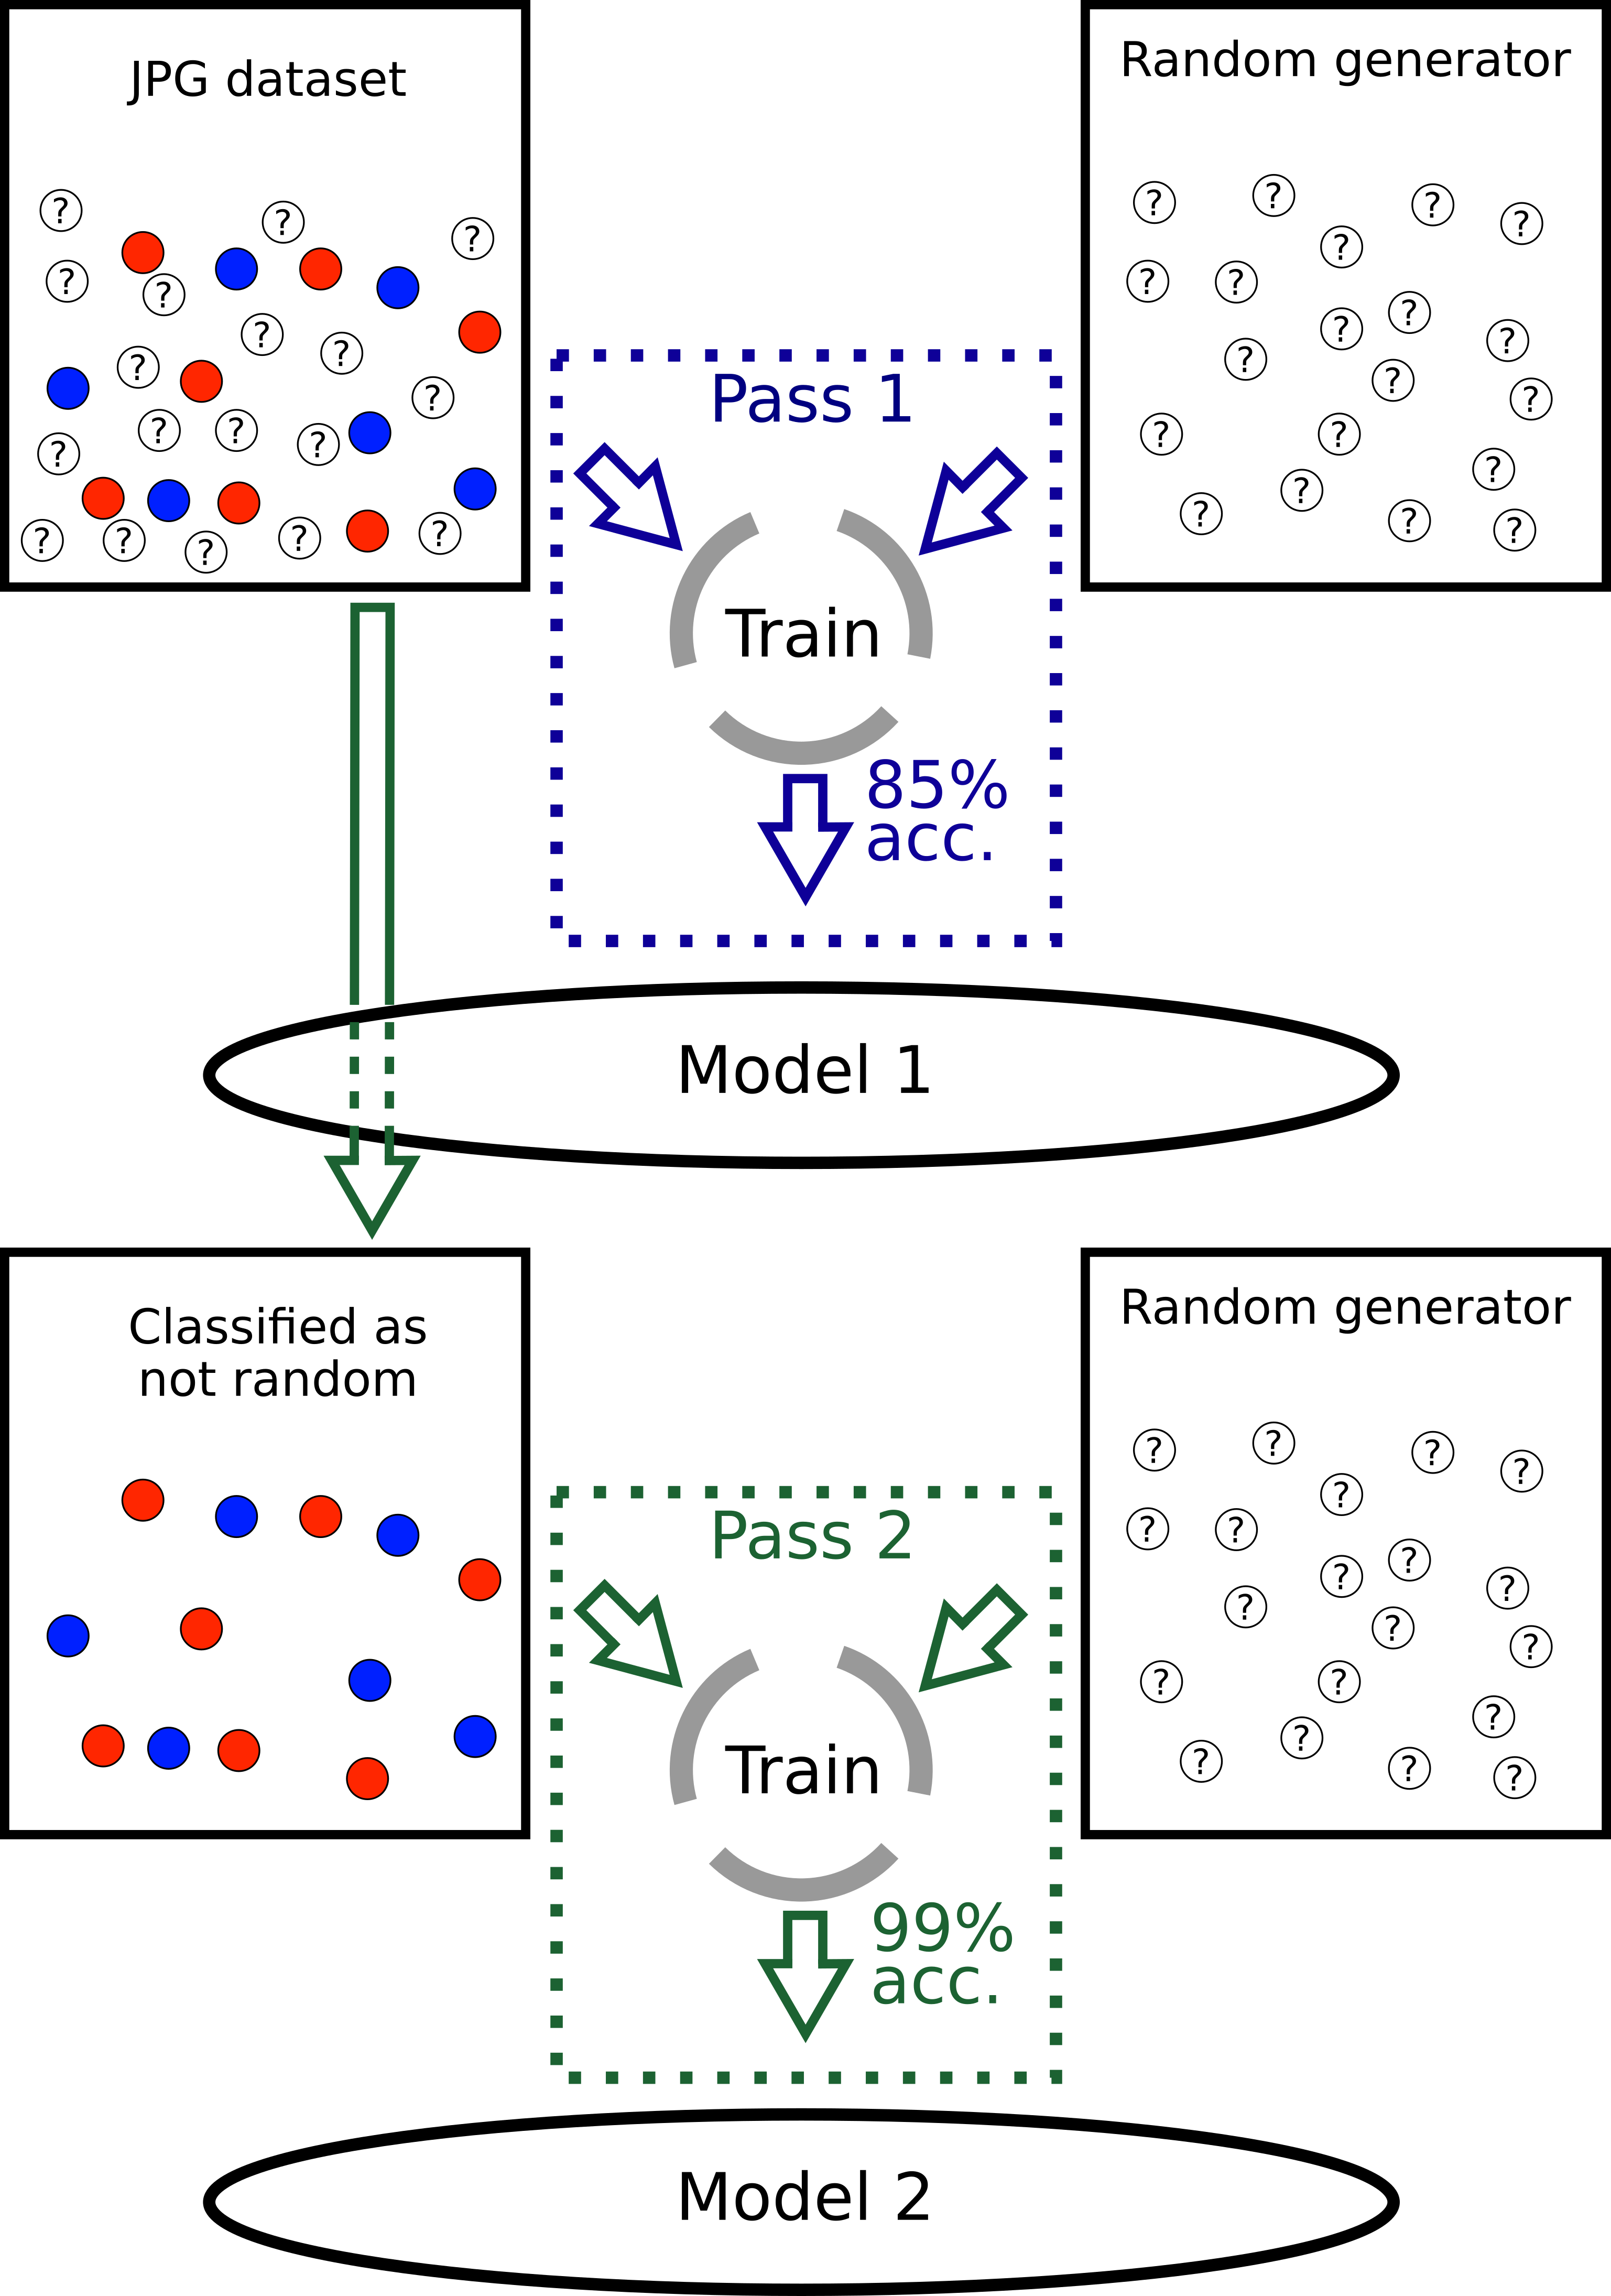
\includegraphics[width=0.5\textwidth]{content/random_measure.png}
\caption{\label{fig:randommeasure}Example of the random measure for the JPG file type. In pass 1, a model is trained to classify the data as ``random'' or ``structured'', achieving 87\% accuracy. In pass 2, another model is trained to do the same task, but the JPG blocks used are those classified as ``structured'' by model 1. As model 2 achieves an accuracy of 99\%, it validates that almost all the blocks classified as ``structured'' by model 1 are indeed not random. Then model 1 can be used to make an upper boundary estimate of the randomness of the dataset.}%
\end{figure*}
\todo[inline]{update figure and label to reflect results}

When the model training finishes the first pass, if the validation accuracy is above a predefined threshold (98\% in this study) for a given file type, no further passes are required by that file type, as the model already can distinguish between ``random'' and ``structured'' classes for that particular file type. This will only happen on file types that have almost no random-like structures.

In the second pass, the file type dataset is filtered and only those fragments classified as ``structured'' in the first pass are used in the second pass. The random generator does not require similar filtering. If in the second pass the accuracy is above the predefined threshold, it means that the first pass successfully selected samples that have almost no random-like structures. In that case, the model of the first pass can then be used in the original dataset, giving a count of how many fragments are correctly identified as ``structured''. In this particular case, the model of the first pass can be used to filter the dataset, hence the method name, as it can split the data with almost no false positives.

If the second pass accuracy is below the threshold, the equations used in the previous section can be used on the results of the second pass, to avoid further passes.



    \levelB{Results}
    % \levelC{Hardware}
The experiments did not take advantage of GPU acceleration and were  conducted on a single computer with 256GB of RAM and with 2 Intel\textregistered Xeon\textregistered E5-2630 v2 processors, with 6 cores each, with 2 hyper-threads per core, or 24 hyper-threads in total. 


% \levelC{Software}
The main software and frameworks used to build the experiments were Python 3.6 
\cite{rossum_python_2019}, Jupyter notebook \cite{perez_jupyter_2019}, Tensorflow 1.14.0 \cite{google_brain_tensorflow_2019}, Keras 2.2.4-tf \cite{chollet_keras_2019}, and Fedora Linux 27.
% repository
The source code for the experiments is available at \sloppy\url{http://github.com/atilaromero/carving-experiments}.


\begin{table}[!ht]
    \centering
    \caption[Complement of entropy measure]{Complement of entropy measure.}
    \label{tab:pass1}
\begin{tabular}{|l|l|l|l|l|l|l|}
\hline
Category & GovdocsACC & RandomACC & Time   & Epochs & GovdocsTP & GovdocsPrec \\ \hline
dwf      & 0.528           & 0.914          & 16m16s & 37     & 0.483589  & 0.915888         \\ \hline
gz       & 0.613           & 0.906          & 16m59s & 37     & 0.572848  & 0.934499         \\ \hline
swf      & 0.592           & 0.970          & 19m58s & 43     & 0.579381  & 0.978685         \\ \hline
kmz      & 0.589           & 0.983          & 16m21s & 36     & 0.581892  & 0.987932         \\ \hline
png      & 0.659           & 0.960          & 19m40s & 46     & 0.644792  & 0.978440         \\ \hline
pdf      & 0.674           & 0.977          & 29m59s & 70     & 0.666325  & 0.988613         \\ \hline
pps      & 0.748           & 0.962          & 26m12s & 57     & 0.738046  & 0.986692         \\ \hline
pptx     & 0.827           & 0.828          & 12m59s & 30     & 0.791063  & 0.956545         \\ \hline
ppt      & 0.827           & 0.977          & 28m18s & 63     & 0.822927  & 0.995075         \\ \hline
gif      & 0.848           & 0.991          & 16m40s & 39     & 0.846620  & 0.998372         \\ \hline
jpg      & 0.865           & 0.990          & 25m31s & 59     & 0.863636  & 0.998424         \\ \hline
doc      & 0.885           & 0.990          & 14m13s & 31     & 0.883838  & 0.998687         \\ \hline
eps      & 0.989           & 1.000          & 8m00s  & 19     & 0.989000  & 1.000000         \\ \hline
ps       & 0.990           & 1.000          & 4m55s  & 11     & 0.990000  & 1.000000         \\ \hline
xls      & 0.991           & 1.000          & 9m51s  & 23     & 0.991000  & 1.000000         \\ \hline
sql      & 0.995           & 1.000          & 5m19s  & 11     & 0.995000  & 1.000000         \\ \hline
kml      & 0.995           & 1.000          & 7m43s  & 16     & 0.995000  & 1.000000         \\ \hline
log      & 0.998           & 1.000          & 5m19s  & 12     & 0.998000  & 1.000000         \\ \hline
wp       & 0.998           & 1.000          & 5m19s  & 11     & 0.998000  & 1.000000         \\ \hline
hlp      & 1.000           & 1.000          & 4m49s  & 11     & 1.000000  & 1.000000         \\ \hline
rtf      & 1.000           & 1.000          & 5m17s  & 12     & 1.000000  & 1.000000         \\ \hline
html     & 1.000           & 1.000          & 5m01s  & 11     & 1.000000  & 1.000000         \\ \hline
f        & 1.000           & 1.000          & 4m50s  & 11     & 1.000000  & 1.000000         \\ \hline
java     & 1.000           & 1.000          & 5m18s  & 11     & 1.000000  & 1.000000         \\ \hline
txt      & 1.000           & 1.000          & 4m42s  & 11     & 1.000000  & 1.000000         \\ \hline
csv      & 1.000           & 1.000          & 5m19s  & 12     & 1.000000  & 1.000000         \\ \hline
xml      & 1.000           & 1.000          & 5m14s  & 11     & 1.000000  & 1.000000         \\ \hline
dbase3   & 1.000           & 1.000          & 4m42s  & 11     & 1.000000  & 1.000000         \\ \hline
\end{tabular}
\end{table}

The results obtained are shown in Table \ref{tab:pass1}. The entropy measure is the complement of the GovdocsTP column.  The GovdocsACC columns contains the accuracy validations values as calculated by Keras on the Govdocs1 dataset, thus considering all samples labeled as ``random'' as errors. The RandomACC column lists the portion of samples from the random generator classified as ``random'' by the model for that file type. The Time and Epoch columns refer to the training session of each model. The GovdocsTP column uses the equation \ref{eq:TPend}, giving the complement of the entropy. GovdocsPrec is simply $GovdocsTP/GovdocsACC$.

Figure \ref{fig:not_random} shows, for each file type, the percent of 512-byte fragments identified as ``structured'', from a sample of 1000 fragments for each file type.
In the figure, the 87\% value for JPG, for example, means that up to 87\% of the blocks of the JPG dataset have recognizable patterns. Since the assumption of no false negatives was used, the real value, which is unknown, can be lower. The entropy measure proposed is the complement of this value, for example, 13\% for JPG.

\noindent
\begin{figure*}[htb!]
\centering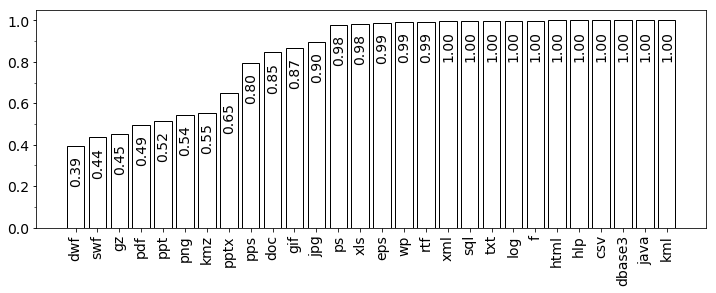
\includegraphics[width=1.0\textwidth]{content/random.png}
\caption[Complement of entropy measure for 28 file types]{\label{fig:not_random}Estimate of the percentage of samples with recognizable structures, using models trained to distinguish each file type from random data. }%
\end{figure*}


    \levelB{Discussion}
    Having a minimum number of recognizable structures for each file type, it is now possible to calculate the maximum number of the classification errors that can be attributed to error cause E1, which happens when the complexity of the data is beyond the model’s capability to recognize patterns.

The mean true positive estimate for all file types, using data listed in figure \ref{fig:not_random}, is 87.3\%.  Assuming a dataset with balanced classes, if all the blocks considered random data were misclassified, then the maximum amount of error due to data complexity would be 12.7\%. If all blocks considered random were classified as DWG, which is the class with less recognizable patterns, then the maximum amount of error would be 10.9\%.

Since the higher validation accuracy obtained in chapter \ref{sec:evalmodels} for these 28 file types using the ``CLD'' models was 0.63, that model has an error rate of 37\%. But only 12.7\% of those errors can be attributed to the error cause E1, which happens when the model is unable to detect structures in the data.

The hypothesis proposed in this chapter is only partially confirmed: some of the errors can be attributed to error cause E1, but only to some extent. About 2/3 of the errors cannot be explained by error cause E1. Since the false negative assumption was used, 2/3 may be an underestimation.


% \levelC{Limitations and threats to validity}
The procedure applied in this experiment uses the no false negative assumption, which considers that no sample with recognizable structures is erroneously classified as ``random''. Thus, it is expected that the exact valid fragment count, which is unknown in practice, will be higher than the number obtained. Taking the JPG file type as an example, in which 87\% of the blocks were identified as ``structured'', this means that the true entropy value would be some unknown value between zero and 13\%.

Also, it is important to notice that the use of different network architectures may result in different measures, as their ability to recognize patterns in the data may be different.


%7
\levelA{\label{chap:conclusion}Conclusion}
{\color{red}
File fragment classification aims to identify the original type of file from which a given block of
data was extracted. Machine learning techniques, and neural networks in particular, have the potential to improve this field, because the support of a new file type using traditional methods is laborious and not automatic. While studies on neural networks applied for file fragment classification have shown good results, to apply those contributions on real scenarios a better understanding is required on how those methods respond to an increase in number of supported file types and what the are the main sources of errors of this approach.
}

The research described in this study was divided into three parts.
In Chapter \ref{sec:evalmodels}, during the search for the best model to classify file fragments, an apparent limit on how far these models could be improved was found. This limitation can be also observed in other works, since training the model ``CLD'' with the same file types used in those works resulted in accuracy values similar to theirs.

In Chapter \ref{sec:numberofclasses}, the influence of the number of classes on accuracy was explored. It was observed that an increase in the number of classes tends to decrease the accuracy and to increase the precision. But the number of classes alone was found to be less important than the type of extension selected: some file types when included in the experiment have a much higher negative impact than others, especially those that use compression or contain images.

In Chapter \ref{sec:exprandom}, a method to measure entropy was proposed. One advantage of this method is that it can be customized to a particular neural network architecture. It was used to measure, for each file type, what portion of the data did not have structures detectable by the chosen model, ``CLD''.

This measure was used to verify the hypothesis that part of the errors observed in Chapter \ref{sec:evalmodels} were caused by high entropy on some file types, as the results of chapter  \ref{sec:numberofclasses} suggested.

The portion of data that could be identified as containing structures was higher than expected. While some of the errors could be explained by the inability of the models to distinguish  high entropy data from random data, this could only explain about 1/3 of the observed errors (12.7\% out of 37\%).

This raises the question of whether the remaining 2/3 of errors could be explained by different file types using the same data structures. This error source comes from the practice of using the extension of the file as the class to each of its parts. An analogy with speech recognition would be to label each syllable of a spoken word using the word as its label and then try to predict the whole word using only a syllable.

Unfortunately, in the file fragmentation task, the potential labels for smaller parts may be less obvious than it is in speech recognition. The best-case scenario would be if the neural network itself could choose the labeling. But evaluating those predicted labels using labels of its own choosing would introduce bias, as it could prefer to create only easy labels.
% The statement that all file types are composed of ``data'' is correct, but it is unhelpful.

An additional contribution of this work is the availability of the source code used to generate the results, which is a feature that not all studies provide. It can be used as a basis of comparison in future researches, generating models with the same architecture of those presented here.
    \levelB{Future work}
    For future research on file fragment classification, the hypothesis that the remaining 2/3 of the observed errors are caused by similar data structures used by multiple files should be explored. Also, the search for a procedure to automatically label inner data structures of files may be a promising strategy. 

Other approaches that can be used inlude 
\todo[inline]{more future works}

\todo[inline]{review references}

% Having recognized the potential of neural networks in the data carving task, there are still some research paths that should be explored.

% \todo[inline]{qual a dificuldade da tarefa de identificacao do tipo de arquivo, o que os outros metodos atingem de acuracia?}

% \todo[inline]{aumentar número de tipos de arquivos suportados}

% \todo[inline]{Existem aspectos que já avançaram mas não citados no texto, por exemplo, já consegue identificar o início e o fim do arquivo.}

% One of them is about the increase in the range of supported filetypes. In a collaborative approach, should the said community be sharing models, datasets, or both? What are the strengths and weakness of each?

% Another one is about reassembling. After each block has been classified, how to reconstruct the original file in the occurrence of fragmentation?

% \todo[inline]{Quanto a remontagem? Existe uma previsão e qual o dataset tu vais utilizar? Como vai conseguir remontar? Este problema é complicado, mas deve tentar avançar de alguma forma.}

% \todo[inline]{Pretende ainda avançar nos tipos de arquivos e na remontagem. Mesmo que não consiga remontar, pelo menos mostrar o que não conseguiu, pois facilita para quem for feito. —> Verificar a literatura se ninguém está fazendo isto mesmo.}

% The last one is about the recognized structures. Is it possible to use the trained networks to describe the structures being recognized?

% ==========


% The following questions are intended to be answered in future works: 

% \begin{enumerate}[itemindent=\parindent,label=\textbf{Q\arabic*.}]

%     \item Could a neural network based tool support a wider range of file types?
    
%     \item Could a neural network based tool handle fragmentation through reassembling?
    
%     % \item Do the results obtained with usual datasets reflect what happens in real scenarios?

% \item Do neural networks help to interpret internal file structures?

% \end{enumerate}

% \todo[inline]{compare solutions - possible candidates: feedforward, convolutional, LSTM, BLSTM, SVM, kNN, Photorec, Foremost, scalpel}
% \todo[inline]{shuffle data to simulate fragmentation}
% \todo[inline]{removal of portions of files to simulate data corruption}
% \todo[inline]{increase the number of supported file types, investigating the best strategy to scale the solution}
% \todo[inline]{reassembling}
% \todo[inline]{model share}
% \todo[inline]{adaption of visualization techniques of neural networks, attempting to infer file structure.}
